% THIS IS AN EXAMPLE DOCUMENT FOR VLDB 2012
% based on ACM SIGPROC-SP.TEX VERSION 2.7
% Modified by  Gerald Weber <gerald@cs.auckland.ac.nz>
% Removed the requirement to include *bbl file in here. (AhmetSacan, Sep2012)
% Fixed the equation on page 3 to prevent line overflow. (AhmetSacan, Sep2012)

\documentclass{vldb}
\usepackage{graphicx}
\usepackage{balance}
\usepackage{ dsfont }
\usepackage{algorithm}
%\usepackage{algorithmic}
\usepackage{listings}
\usepackage{algorithmicx}
\usepackage{subfigure}
\usepackage{algpseudocode}
\algnotext{EndFor}
\algnotext{EndIf}
\usepackage{color}
\usepackage{comment}
\usepackage[htt]{hyphenat}
\usepackage{mathtools}
\usepackage{hyperref}

\usepackage[font={small,it}]{caption}

\DeclarePairedDelimiter\ceil{\lceil}{\rceil}
\DeclarePairedDelimiter\floor{\lfloor}{\rfloor}
\specialcomment{edit}{\begingroup\sffamily\color{blue}}{\endgroup}
% for  \balance command ON LAST PAGE  (only there!)


\begin{document}

% ****************** TITLE ****************************************

\title{Rasterized Image Databases with LSH\\
for Compression, Search and Duplicate Detection}

% possible, but not really needed or used for PVLDB:
%\subtitle{[Extended Abstract]
%\titlenote{A full version of this paper is available as\textit{Author's Guide to Preparing ACM SIG Proceedings Using \LaTeX$2_\epsilon$\ and BibTeX} at \texttt{www.acm.org/eaddress.htm}}}

% ****************** AUTHORS **************************************

% You need the command \numberofauthors to handle the 'placement
% and alignment' of the authors beneath the title.
%
% For aesthetic reasons, we recommend 'three authors at a time'
% i.e. three 'name/affiliation blocks' be placed beneath the title.
%
% NOTE: You are NOT restricted in how many 'rows' of
% "name/affiliations" may appear. We just ask that you restrict
% the number of 'columns' to three.
%
% Because of the available 'opening page real-estate'
% we ask you to refrain from putting more than six authors
% (two rows with three columns) beneath the article title.
% More than six makes the first-page appear very cluttered indeed.
%
% Use the \alignauthor commands to handle the names
% and affiliations for an 'aesthetic maximum' of six authors.
% Add names, affiliations, addresses for
% the seventh etc. author(s) as the argument for the
% \additionalauthors command.
% These 'additional authors' will be output/set for you
% without further effort on your part as the last section in
% the body of your article BEFORE References or any Appendices.

\numberofauthors{4} %  in this sample file, there are a *total*
% of EIGHT authors. SIX appear on the 'first-page' (for formatting
% reasons) and the remaining two appear in the \additionalauthors section.

\author{
% You can go ahead and credit any number of authors here,
% e.g. one 'row of three' or two rows (consisting of one row of three
% and a second row of one, two or three).
%
% The command \alignauthor (no curly braces needed) should
% precede each author name, affiliation/snail-mail address and
% e-mail address. Additionally, tag each line of
% affiliation/address with \affaddr, and tag the
% e-mail address with \email.
%
% 1st. author
\alignauthor
Zoya Bylinskii\\
       \affaddr{MIT CSAIL}
% 2nd. author
\alignauthor
Maria Shugrina\\
\affaddr{MIT CSAIL}
\and  % use '\and' if you need 'another row' of author names
% 3rd. author
\alignauthor
Andrew Spielberg\\
       \affaddr{MIT CSAIL}
% 4th. author
\alignauthor
Wei Zhao\\
\affaddr{MIT CSAIL}
}
\date{\today}
% Just remember to make sure that the TOTAL number of authors
% is the number that will appear on the first page PLUS the
% number that will appear in the \additionalauthors section.


\maketitle

\begin{abstract}
We present a novel strategy for patch-based lossy compression which exploits the inevitable redundancy found in large image collections.  We describe a scalable PostgreSQL-based implementation leveraging the indexing infrastructure found in relational DBMS.  We decompose images into sets of \emph{patches} which we define to be small contiguous subregions of images.  Since many image textures (e.g. sky, ocean, forest, walls, etc.) are ubiquitous in image datasets, rather than store all the information of these patches for every image, we only store pointers to approximating patches in a \emph{patch dictionary}.  This dictionary is grown in an online fashion as new images are added, in the case where no similar-enough patch can currently be found in the database under our chosen patch distance function.  In order to efficiently retrieve patches from our database, we make use of Locality-Sensitive Hashing and a number of key optimizations.  We analytically compute the savings of our compression scheme, and experimentally demonstrate its performance over various image categories of the large SUN 2012 database. Finally, we provide subjective and quantitative evaluations of our compression quality.
\end{abstract}


\section{Introduction}

Large collections of images are ubiquitous in the modern digital world.
According to one 2014 Internet Trends report,
more than 1.8 billion images are uploaded to the internet every day~\cite{meeker2014internet}.
Our work is inspired by the intuition that there must be a lot of redundancy
in large image collections, and that this redundancy could
be exploited for more efficient storage and for applications such as duplicate detection.

We focus on image redundancy on the patch level, assuming that large collections
of images must have many patches which are nearly the same.
Our goal is to store a set of images as a database of
similar patches, where similar patches may be shared between images,
 such that we minimize the storage space while maintaining certain \emph{quality}
of reconstructed images. In effect, this results in lossy compression. More concretely,
we aim to choose patch similarity criterion, and search and reconstruction algorithms such
that:
\begin{itemize}
\item the database size is smaller than if full images were stored
\item the images can be reconstructed from the database in real time
\item the reconstructed images fulfill certain quality requirements (See Sec.~\ref{ssec:qual-met})
\end{itemize}
These conflicting introduce a number of tradeoffs, such as size of
the database versus image quality.
The goal of this paper is as much to produce a working system as to
build up the analytical foundations that allow making these tradeoffs.

In Section~\ref{sec:method}, we explain our method of ``patchifying'' images,
storing them in a database, and reconstructing stored images. We also
discuss image similarity, hashing schemes and indices in this core section.
In Section~\ref{sec:analysis}, we provide analytical groundwork for
selecting optimal image patch sizes, similarity threshold, and the quality metrics
appropriate for evaluation. Finally, in Section~\ref{sec:performance}
we evaluate our system on real data, using analytical tools from the previous section.
In addition, in Section~\ref{sec:apps}, we briefly touch on applications that come naturally
from a patch database, including similar image retrieval and duplicate detection.

\section{Related Work}\label{sec:related}

Lossless image compression techniques like \emph{area coding} or \emph{Huffman coding} give quality guarantees but do not always give sufficient savings (especially for unstructured images). Lossy image compression algorithms, on the other hand, are quite popular and used for most applications dealing with natural images, including storage in image datasets, and web transmission. Often, lossy compression depends on a quantization of image regions (e.g. all pixels in a block of the image receive the same color value). For instance, the \emph{JPEG compression} standard partitions an image into non overlapping blocks and applies a discrete cosine transform to each block, quantizing the resulting coefficients. \emph{Fractal compression} techniques \cite{Jacquin} apply an iterative algorithm to images to encode images as fractal codes, capable of representing different parts of the images at different levels of detail. This algorithm makes use of self-similarities and is computationally expensive. However, due to fast decoding, it can be used for file downloads. All of these approaches, however, operate on a \emph{within-image} basis, compressing an image using either a pre-specified dictionary (quantization) or using within-image similarity. Thus, these approaches provide constant savings for image databases of arbitrary sizes.

In the age of big data, when the amount of images in image collections grows at enormous rates, a compression scheme that scales with the database size seems most appropriate. Thus, we are interested in compression schemes that take into account \emph{across-image} redundancy, not just \emph{within-image} redundancy. 

Some of our inspiration comes from \emph{raster databases}, which encode images (often of geospatial data) as a set of smaller images/regions with locations in the original large image. Such a set-up is convenient for transmission or data loading, as it is possible to load and process only parts of the image at a time. Geodatabases, such as \emph{ArcGIS} are set-up this way \cite{ArcGIS}.

We combine the idea of raster databases with the idea of image compression. Patch-based image representations are also used in computer vision for various tasks, including image matching \cite{Brown05}, object recognition \cite{vashist2006dps}, and image processing \cite{Barnes2009}. Considering images as collections of patches allows for arbitrary spatial matching. 

\begin{edit}

Image similarity functions.

Image quality functions.

Hashing, in particular~\cite{LSH:Andoni}.

\end{edit}
\section{Method}\label{sec:method}

To limit the complexity, we assume
each image to be a square of $m^2$ pixels, and for all patches to
be squares of the same size.
We formally describe our method in Sec.~\ref{ssec:overview}. To summarize,
we first segment each image into patches and store them in the \texttt{patches} database.
Only patches sufficiently different
from all the patches in \texttt{patches} are stored (See Sec.~\ref{ssec:sim}).
Instead of storing each image explicitly, we approximate it by storing pointers to the patches
approximating its original patches. In Sec.~\ref{ssec:lsh}, we describe the
search algorithm used to quickly retrieve similar patches, and in Sec.~\ref{ssec:reconst}
we detail the indices that make image reconstruction faster. Finally, in
Sec.~\ref{ssec:impl} we provide implementation details.

\subsection{Overview}\label{ssec:overview}

Our method is governed by the following parameters:
\begin{itemize}
\item $n$ - width and height of all patches\footnote{We assume that $m \mod n$ is $0$.}
\item $S$ - similarity function from two $n \times n$ images to $\mathbb{R}$
\item $T$ - similarity threshold
\end{itemize}
The $n \times n$ patches are stored as byte data in the \texttt{patches} table.
To allow image reconstruction, we also store $(m / n)^2$ patch pointers for
each image in the \texttt{patch\_pointers} table. The full schema looks as follows:
\begin{verbatim}
patches(id int PRIMARY KEY,
        patch bytea);

images(imgid int PRIMARY KEY);

patch_pointers(imgid int REFERENCES images(imgid),
               patch_id int REFERENCES patches(id),
               x int,
               y int);
\end{verbatim}
where \texttt{patch\_pointers.x} and \texttt{patch\_pointers.y}
refer to the left top corner location of each patch in the image.

Given these tables, inserting an image into the database proceeds as follows:

\begin{algorithm}
    \caption{Insert Image $I$ into database}
    \label{alg:insert}
\begin{algorithmic}[1]
\State $Patches \leftarrow $ \texttt{CutIntoPatches}(I, patch\_size=$n$)
\For{$P$ in $Patches$}
\State $SimPat \leftarrow $\texttt{FindLikelySimilarPatches}($P$)
\State $P_{closest} \leftarrow $ $argmin \{ S(P, P_i) \}$
\If $S(P, P_i) > T$
\State \texttt{insert} $P$ into \texttt{patches}
\EndIf
\EndFor
\vspace{3mm}
\end{algorithmic}
\end{algorithm}
Sections \ref{ssec:sim} and \ref{ssec:lsh} detail similarity measure and
finding patches that are likely to be similar.

In order to reconstruct an image from that patches, we run the following
procedure:



\subsection{Patch Similarity}\label{ssec:sim}
There are many image similarity metrics that have been developed for
images (See~\cite{yasmin2013use} for a good survey.), and
our method is applicable to any metric that involves Euclidean
distance over image features, its stacked color channel pixel values
being the simplest case.

For the purpose of this project, we choose to use squared Euclidean
distance over (CIE)LUV color space.
Given two $n \times n$ patches $P_1$ and $P_2$, we evaluate similarity $S$
per color channel $i$ as follows:

\begin{displaymath}
S(P_1, P_2, i) = \frac{||P_1(i) - P_2(i)||^2}{n^2}
\end{displaymath}
where $||\cdot||$ denotes standard Euclidean norm.
We normalize by the dimensionality of the space to allow us to keep the
similarity threshold independent of the patch size. See section \ref{sec:simthresh} for more details.

The use of Euclidean distance for patch similarity
allows us to use Locality Sensitive Hashing to retrieve patches
that are likely to be similar, as detailed in the
next section.

\subsection{LSH for Patches}\label{ssec:lsh}

\subsection{Image Reconstruction}\label{ssec:reconst}

In order to reconstruct images quickly, we

\subsection{Implementation}\label{ssec:impl}
We used $postgresql$ to construct our database, and used
Java API to talk to the database from a custom executable. Locality
sensitive hashing, image segmentation and reconstruction were
all implemented in Java, and used to construct a hash table
on patches in $postbresql$.

Our code is available at:
\begin{verbatim}
https://github.com/shumash/db_project
\end{verbatim}

\section{Near Neighbor Search}\label{sec:nn}

Fast retrieval of similar patches is crucial for making
construction of a sizable patch-based database feasible.
This is essentially near-neighbor retrieval in
relatively high dimensions $3 \cdot n^2$ (1875 for patch size $n=25$).
Image retrieval has been addressed in a number of papers,
including more complex feature representations ~\cite{perronnin2010large}.
Our problem is somewhat different from most of previous work
in that the variability
in small patches is much less than in regular-sized images,
semantic information is irrelevant, and vectors are much shorter
than for regular-sized images.
Thus, we focus on tuning a simple Locality-Sensitive Hashing variant for our
particular application.

\subsection{Locality-Sensitive Hashing}

\begin{figure}[ht!]
\centering
\subfigure[Typical LSH uses several tables.]{
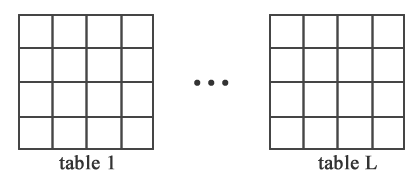
\includegraphics[width=3.0in]{fig_NN/lsh_tables.png}}
\subfigure[Random projection hashing family $\mathcal{F}$.]{
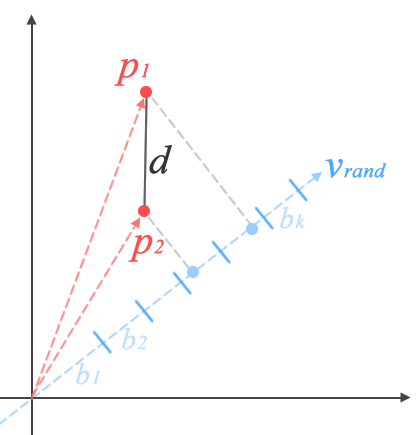
\includegraphics[width=2.5in]{fig_NN/rand_proj.png}}
\caption{a) LSH typically constructs
$L$ hash tables, each relying on an amplified
hash function $\mathcal{G}$, composed of a concatenation
of simpler hash functions $\mathcal{F}$. b) In
random projection hashing, each
$\mathcal{F}$ is evaluated by projecting a point $p$
(a patch color vector in our case) on a randomly chosen
unit vector, and binning it into uniform bins.}
\label{fig:lsh}
\end{figure}

Locality-Sensitive Hashing (LSH)~\cite{LSH:Andoni}
is a popular approach for approximate near-neighbor search
in high dimensions. The high-level idea behind LSH is
using a set of hashing functions that map
a vector $P_i$ to its bin $b(P_i)$ such that:
\begin{equation*}
\begin{aligned}
P[b(P_i) = b(P_j) | S(P_i, P_j) < T] > P_1\\
P[b(P_i) = b(P_j) | S(P_i, P_j) > cT] < P_2
\end{aligned}
\end{equation*}
where the collision probability
for vectors that are close together is high
($> P_1$), and the probability of collision
for vectors that are further apart is low ($< P_2$).

To achieve high guarantees on finding the nearest
neighbor, LSH typically requires multiple hash tables.
For example, two red points in Fig.~\ref{fig:lsh} are close,
but they fall in different bins in table 1. However,
in some table (say Table $L$), they are likely to end up in
the same bin. This amounts to taking an OR over
collisions in all the tables, amplifying probabilities.
Implementing this scenario in the context
of a database incurs a significant overhead, as for each
patch $P_i$ we not only need to store the patch itself,
but also $L$ hash indices. At near neighbor search time,
queries must be made to all the hash tables, which incurs significant
overhead in the database setting.

High precision near neighbor search is not necessary
for our application, and we focus, instead, on \emph{efficiency}.
In order to accomplish that we aim to \textbf{minimize the
probability of collision for dis-similar patches}, as long
as probability of collision for similar patches results in
finding enough neighbors for a suitable compression ratio.
To this end, we aim to answer the question:
\emph{how well can the system perform with just one hash table?}

In order to optimize the performance of our single hash table,
we want to \emph{amplify} the probability of a single hash
function from a family $\mathcal{F}$ by using an AND operator
on collisions with several hash functions
$\mathcal{F}_1...\mathcal{F}_q$ from that family.
This is a standard technique which results in an amplified
hash function $\mathcal{G}$:
\begin{equation}
\mathcal{G}(P_i) = \mathtt{ConcatBits}(\mathcal{F}_1(P_i),...,\mathcal{F}_q(P_i))
\end{equation}\label{eq:ampl}
where $\mathtt{ConcatBits}$ simply allows a constant
number of bits to each hash and concatenates them into a single value.
The probability that dis-similar patches collide with
this amplified function is $(P_2)^q$, where $P_2$ is the
probability of collision using just one function in the family.
We formalize our Near Neighbor search in Sec.~\ref{ssec:nn-lsh},
and take a closer look at hashing functions in the following sections.
In Sec.~\ref{ssec:naive-nn}, we introduce a common choice for a
 hash function family $\mathcal{F}$, and
and optimize it for our application in Sec.~\ref{ssec:pca-nn}
and \ref{ssec:uni-nn}.

\subsection{Near-Neighbor Search with LSH}\label{ssec:nn-lsh}

Using a single amplified hash function $\mathcal{G}$, finding
all likely neighbors of a patch simply amounts to computing
its hash value and taking all the patches that fall into the
same hash bin.
Moreformally, we can define the function
in Alg.~\ref{alg:insert2} as follows:
\begin{algorithmic}[1]
\Statex \texttt{\textbf{FindLikelySimilarPatches}}($P_j$):
\State $h \leftarrow \mathcal{G}$ (\texttt{ToVector($P_j$)})
\State $SimPat \leftarrow$ \texttt{select patch from patch\_dict where id in
(select patch\_id from patch\_hashes where hash = h)}
\end{algorithmic}
Of course, the quality of the result depends heavily on the
properties of the hash function, which is something we discuss next.

\subsection{Random Projections Hashing}\label{ssec:naive-nn}

A common choice for a hash function family $\mathcal{F}$ is
the family of random projection functions. In this scheme,
a given $\mathcal{F}_i(P_j) \in \mathcal{F}$ is evaluated by
projecting $P_j$ onto a randomly chosen unit vector $v_i$,
and binning the value into a randomly chosen bin (See Fig.~\ref{fig:lsh},
where bins are uniform across dot product values:
\begin{equation}
\mathcal{F}_i(P_j) = \floor{\frac{P_i \cdot \mathbf{v}_i + b}{w}}
\end{equation}
We choose to work with this approach, but operate under
the constraint that the value of the amplified $\mathcal{G}$ of $q$
functions $\mathcal{F}_i \in \mathcal{F}$ must fit in a 32-bit int.
This only affords us $10$ hashes in our amplification,
with a bin size of $8$ (3 bits).

It is unlikely that the projection vector picked randomly
will have desirable properties, given high dimensions. For example,
it is quite likely that typical patches will be orthogonal to
most vectors picked, causing many dis-similar patches to
end up in the same bin (and this is exactly the behavior
we observed in our results).

\subsection{PCA-based Projection Hashing}\label{ssec:pca-nn}

\begin{figure}[ht!]
\centering
\subfigure[PCA-based hashing]{%
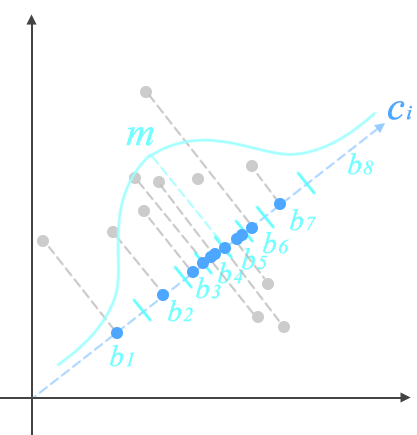
\includegraphics[width=2.5in]{fig_NN/pca_proj.png}
\label{fig:pca-proj}}
\qquad
\subfigure[Dot product distributions]{
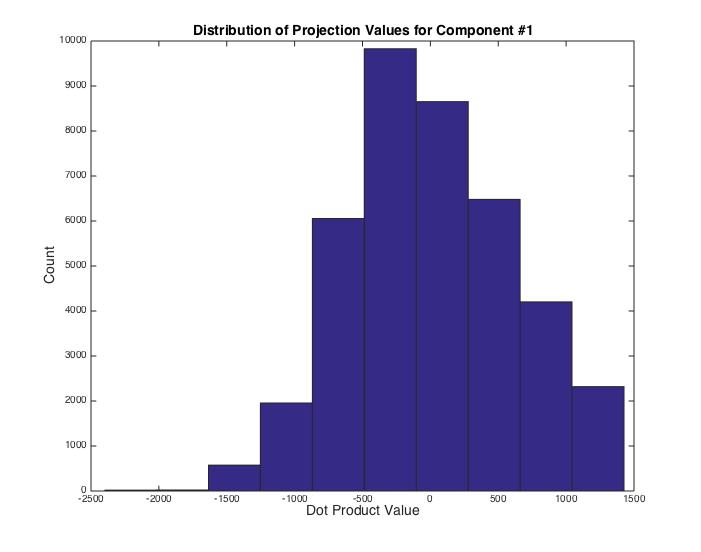
\includegraphics[width=1.0in]{fig_NN/hist_pp1.jpg}
%\vspace{2ex}
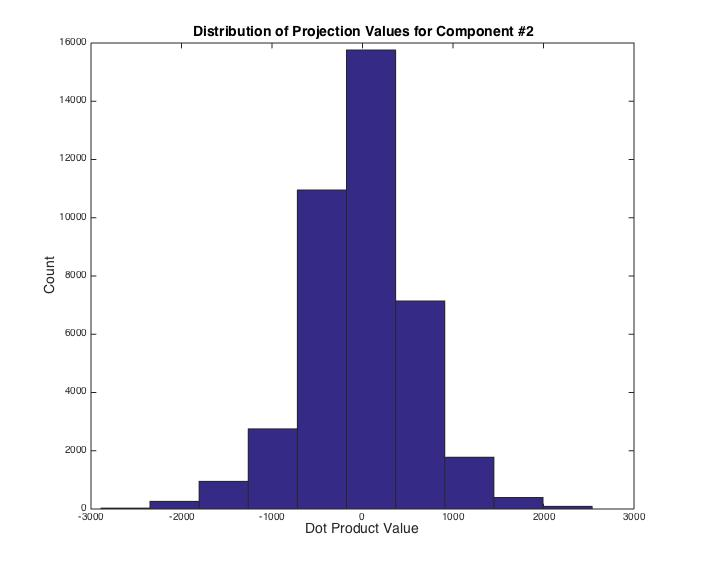
\includegraphics[width=1.0in]{fig_NN/hist_pp2.jpg}
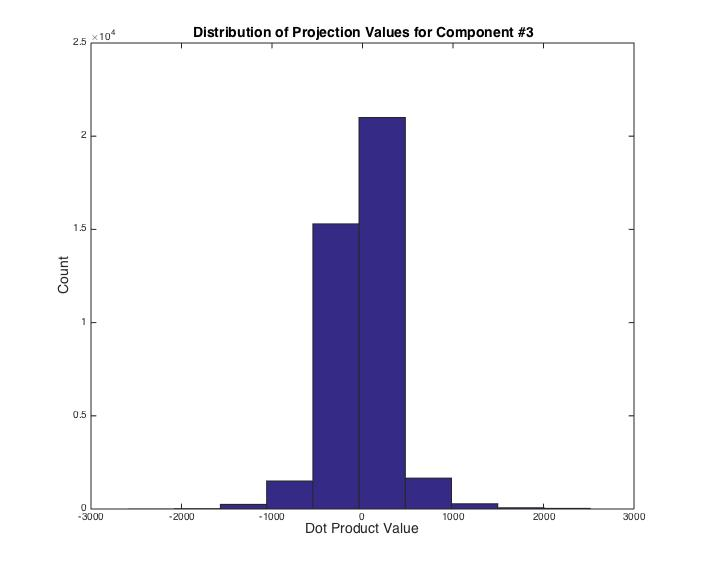
\includegraphics[width=1.0in]{fig_NN/hist_pp3.jpg}
\label{fig:pca-distr}
}
\caption{PCA-based hashing uses directions of maximal
variance in patches as projection vectors, and
adapt the bin size for each projection vector using data.
In b) we show distributions of patch vector projections
on the 3 principal components (magnitude of dot product).}
\label{fig:pca}
\end{figure}

To ensure that patches are well-distributed
among the bins, avoiding database lookup of many potential
neighbors, we propose a \emph{PCA-based hashing scheme}.
Under this scheme, we run Principal Component Analysis (PCA)
to compute directions of largest variance for typical image patches
and use 10 first principal components as the projection
directions (See Fig.~\ref{fig:pca}). This ensures that
the projections of typical patches are as far apart as possible.
To further optimize the binning, we project
a set of patches (grey dots in Fig.~\ref{fig:pca}) onto each
of principal component $\mathbf{v}_i$ (blue dots in Fig.~\ref{fig:pca}), and
approximate the distribution of the dot product
values by a Gaussian $\mathcal{N}_i(\mu_i, \sigma_i)$
(blue curve in Fig.~\ref{fig:pca}).
In order to bin a dot product value into one of 8 bins (3 bits/bin),
we adapt the bin size to $\mu_i$ and $\sigma_i$.

\begin{figure}[ht!]
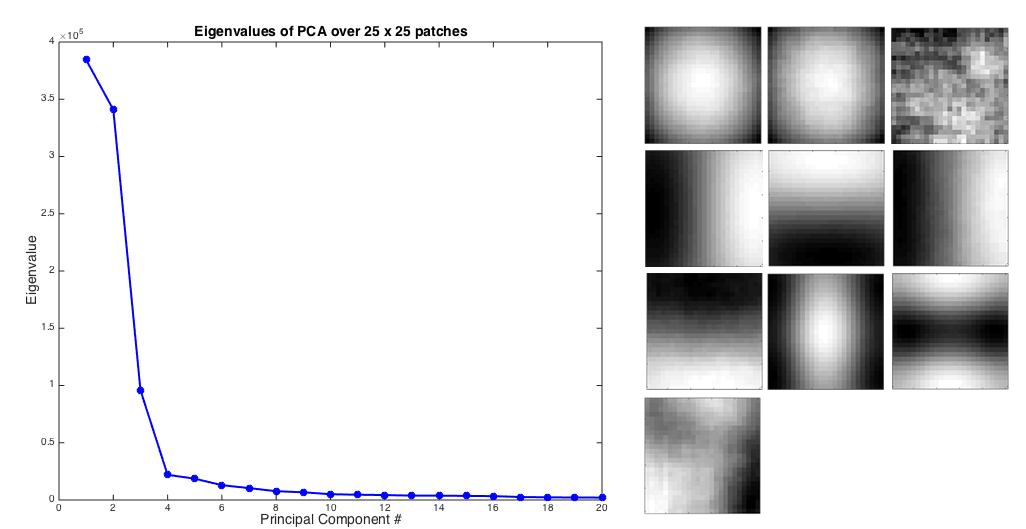
\includegraphics[width=3.0in]{fig_NN/principal_comps.png}
\caption{Eigenvalues of the PCA on 80K patches and visualization
of the L-channel (lightness) of the first 10 components.}
\label{fig:lambdas}
\end{figure}

In our experimental setup we sampled patches from two distinct
sets of 1000 images sampled uniformly from the SUN~\cite{SUN} database
(and distinct from the set of images we inserted into the database),
and used the patches to:
\begin{itemize}
\item compute PCA vectors in Luv color scheme on the \texttt{train{\allowbreak} set}
of 80,000 25x25 patches (See Fig.~\ref{fig:lambdas})
\item compute distribution of typical projections on 10
first principal components using the \texttt{dev{\allowbreak} set} of
40,000 25x25 patches (See Fig.~\ref{fig:pca-distr}).
\end{itemize}
We found that this choice of a hashing function has \emph{a
significant positive effect on performance}(See Sec.~\ref{sec:performance}).

\begin{figure}[ht!]
\subfigure[Pitfalls of standard deviation]{
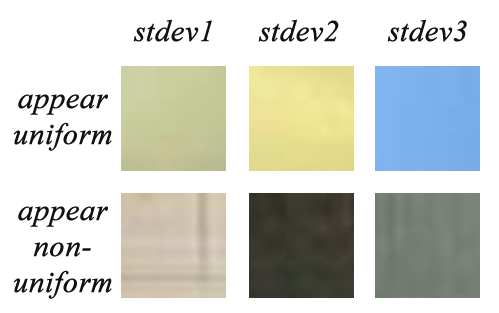
\includegraphics[width=2.5in]{fig_NN/std_uni.png}
\label{fig:color-stdev}}
\subfigure[Uniformity classification with p-norm]{
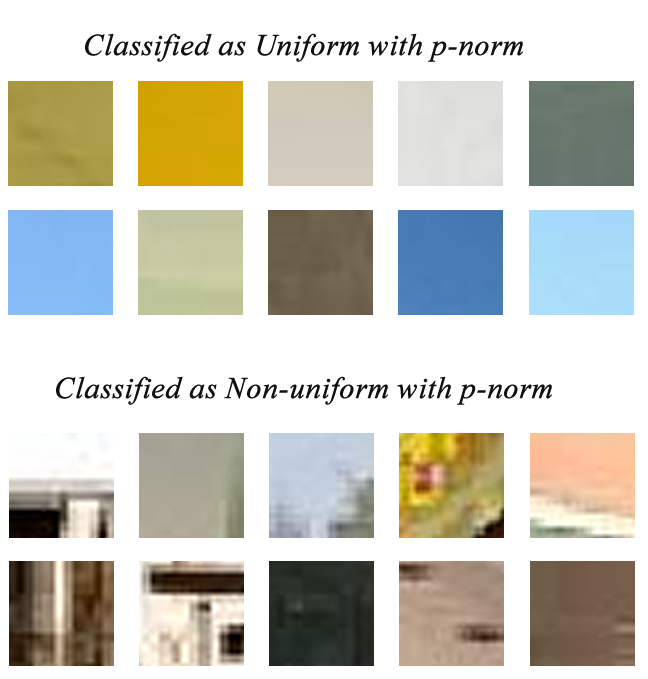
\includegraphics[width=3.0in]{fig_NN/uni_class.png}
\label{fig:color-pnorm}}
\caption{Standard deviation in a) is not very sensitive
to outliers, as patches with nearly identical
values of $stdev1$, $stdev2$ and $stdev3$ may appear
either uniform or non-uniform, as shown in the table.
In b), our classification of patches using
p-norm anecdotally shows more reliable results.}
\end{figure}

\subsection{Hashing Uniform Patches}\label{ssec:uni-nn}

The difficulty of Near Neighbor search for images arises from
their high dimensionality. However, natural images contain many uniform
or nearly uniform patches, which can be easily indexed using
their quantized color. We experimented with using a different
hashing scheme for patches that are nearly uniform, quantizing
them into fewer than 1000 bins by the mean color.

In order to determine if patch $P$ is uniformly colored, we first
looked at the standard deviation $u_2$ of the patch in all channels, which is
just the L-2 norm of $P-\mu(P)$, where $\mu{P}$ is a patch
with every pixel set to the mean of $P$.
However, we found that the L-2 norm is in-sensitive to outliers
(which are very apparent in color patches),
and patches with similar $u_2$ values could appear both uniform
and not-uniform (See Fig.~\ref{fig:color-stdev}).

Instead, we decided to classify uniformity using $u_4$, an L-4 norm
of $P-\mu(P)$, split into channels. Higher order forms tend
to collapse all values $< 1.0$ to zero, and expand all values $> 1.0$
to infinity. Hence, we normalize the elements of $P-\mu(P)$ by
our channel threshold $T$ to ensure this property. The best
approach would pick uniformity thresholds on $u_4$ using
a training set, but in the interests of time we hand-picked
a threshold of $0.1$ for all the channels. See Fig.~\ref{fig:color-pnorm}
for results of this classification on a random set of patches.

We evaluate the performance of PCA-based hashing compared to
a hybrid PCA+uniform patch hashing in Sec.~\ref{sec:performance}.

\section{Performance Optimization}

\section{Near Neighbor Search}\label{sec:nn}

Fast retrieval of similar patches is crucial for making
construction of a sizable patch-based database feasible.
This is essentially near-neighbor retrieval in
relatively high dimensions $3 \cdot n^2$ (1875 for patch size $n=25$).
Image retrieval has been addressed in a number of papers,
including more complex feature representations ~\cite{perronnin2010large}.
Our problem is somewhat different from most of previous work
in that the variability
in small patches is much less than in regular-sized images,
semantic information is irrelevant, and vectors are much shorter
than for regular-sized images.
Thus, we focus on tuning a simple Locality-Sensitive Hashing variant for our
particular application.

\subsection{Locality-Sensitive Hashing}

\begin{figure}[ht!]
\centering
\subfigure[Typical LSH uses several tables.]{
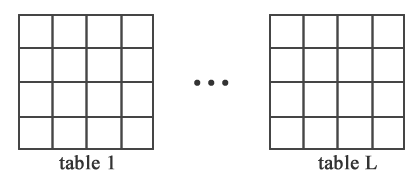
\includegraphics[width=3.0in]{fig_NN/lsh_tables.png}}
\subfigure[Random projection hashing family $\mathcal{F}$.]{
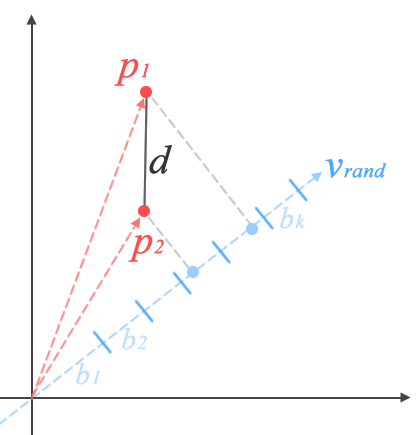
\includegraphics[width=2.5in]{fig_NN/rand_proj.png}}
\caption{a) LSH typically constructs
$L$ hash tables, each relying on an amplified
hash function $\mathcal{G}$, composed of a concatenation
of simpler hash functions $\mathcal{F}$. b) In
random projection hashing, each
$\mathcal{F}$ is evaluated by projecting a point $p$
(a patch color vector in our case) on a randomly chosen
unit vector, and binning it into uniform bins.}
\label{fig:lsh}
\end{figure}

Locality-Sensitive Hashing (LSH)~\cite{LSH:Andoni}
is a popular approach for approximate near-neighbor search
in high dimensions. The high-level idea behind LSH is
using a set of hashing functions that map
a vector $P_i$ to its bin $b(P_i)$ such that:
\begin{equation*}
\begin{aligned}
P[b(P_i) = b(P_j) | S(P_i, P_j) < T] > P_1\\
P[b(P_i) = b(P_j) | S(P_i, P_j) > cT] < P_2
\end{aligned}
\end{equation*}
where the collision probability
for vectors that are close together is high
($> P_1$), and the probability of collision
for vectors that are further apart is low ($< P_2$).

To achieve high guarantees on finding the nearest
neighbor, LSH typically requires multiple hash tables.
For example, two red points in Fig.~\ref{fig:lsh} are close,
but they fall in different bins in table 1. However,
in some table (say Table $L$), they are likely to end up in
the same bin. This amounts to taking an OR over
collisions in all the tables, amplifying probabilities.
Implementing this scenario in the context
of a database incurs a significant overhead, as for each
patch $P_i$ we not only need to store the patch itself,
but also $L$ hash indices. At near neighbor search time,
queries must be made to all the hash tables, which incurs significant
overhead in the database setting.

High precision near neighbor search is not necessary
for our application, and we focus, instead, on \emph{efficiency}.
In order to accomplish that we aim to \textbf{minimize the
probability of collision for dis-similar patches}, as long
as probability of collision for similar patches results in
finding enough neighbors for a suitable compression ratio.
To this end, we aim to answer the question:
\emph{how well can the system perform with just one hash table?}

In order to optimize the performance of our single hash table,
we want to \emph{amplify} the probability of a single hash
function from a family $\mathcal{F}$ by using an AND operator
on collisions with several hash functions
$\mathcal{F}_1...\mathcal{F}_q$ from that family.
This is a standard technique which results in an amplified
hash function $\mathcal{G}$:
\begin{equation}
\mathcal{G}(P_i) = \mathtt{ConcatBits}(\mathcal{F}_1(P_i),...,\mathcal{F}_q(P_i))
\end{equation}\label{eq:ampl}
where $\mathtt{ConcatBits}$ simply allows a constant
number of bits to each hash and concatenates them into a single value.
The probability that dis-similar patches collide with
this amplified function is $(P_2)^q$, where $P_2$ is the
probability of collision using just one function in the family.
We formalize our Near Neighbor search in Sec.~\ref{ssec:nn-lsh},
and take a closer look at hashing functions in the following sections.
In Sec.~\ref{ssec:naive-nn}, we introduce a common choice for a
 hash function family $\mathcal{F}$, and
and optimize it for our application in Sec.~\ref{ssec:pca-nn}
and \ref{ssec:uni-nn}.

\subsection{Near-Neighbor Search with LSH}\label{ssec:nn-lsh}

Using a single amplified hash function $\mathcal{G}$, finding
all likely neighbors of a patch simply amounts to computing
its hash value and taking all the patches that fall into the
same hash bin.
Moreformally, we can define the function
in Alg.~\ref{alg:insert2} as follows:
\begin{algorithmic}[1]
\Statex \texttt{\textbf{FindLikelySimilarPatches}}($P_j$):
\State $h \leftarrow \mathcal{G}$ (\texttt{ToVector($P_j$)})
\State $SimPat \leftarrow$ \texttt{select patch from patch\_dict where id in
(select patch\_id from patch\_hashes where hash = h)}
\end{algorithmic}
Of course, the quality of the result depends heavily on the
properties of the hash function, which is something we discuss next.

\subsection{Random Projections Hashing}\label{ssec:naive-nn}

A common choice for a hash function family $\mathcal{F}$ is
the family of random projection functions. In this scheme,
a given $\mathcal{F}_i(P_j) \in \mathcal{F}$ is evaluated by
projecting $P_j$ onto a randomly chosen unit vector $v_i$,
and binning the value into a randomly chosen bin (See Fig.~\ref{fig:lsh},
where bins are uniform across dot product values:
\begin{equation}
\mathcal{F}_i(P_j) = \floor{\frac{P_i \cdot \mathbf{v}_i + b}{w}}
\end{equation}
We choose to work with this approach, but operate under
the constraint that the value of the amplified $\mathcal{G}$ of $q$
functions $\mathcal{F}_i \in \mathcal{F}$ must fit in a 32-bit int.
This only affords us $10$ hashes in our amplification,
with a bin size of $8$ (3 bits).

It is unlikely that the projection vector picked randomly
will have desirable properties, given high dimensions. For example,
it is quite likely that typical patches will be orthogonal to
most vectors picked, causing many dis-similar patches to
end up in the same bin (and this is exactly the behavior
we observed in our results).

\subsection{PCA-based Projection Hashing}\label{ssec:pca-nn}

\begin{figure}[ht!]
\centering
\subfigure[PCA-based hashing]{%
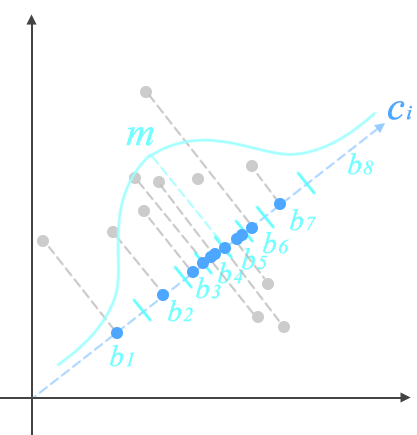
\includegraphics[width=2.5in]{fig_NN/pca_proj.png}
\label{fig:pca-proj}}
\qquad
\subfigure[Dot product distributions]{
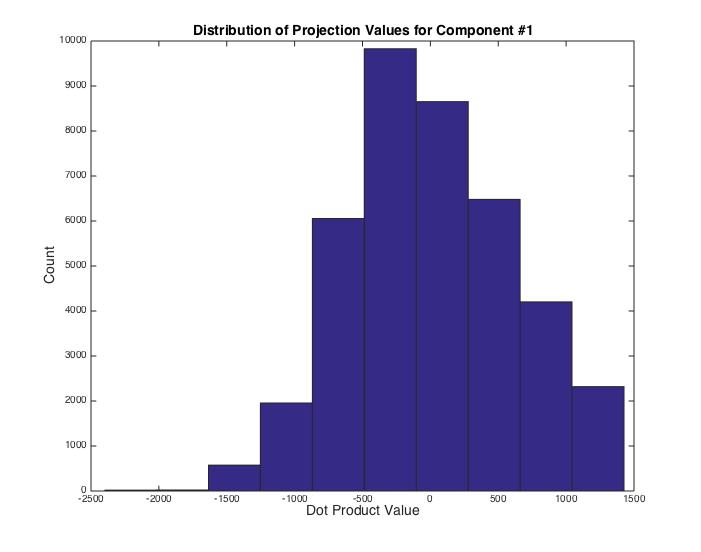
\includegraphics[width=1.0in]{fig_NN/hist_pp1.jpg}
%\vspace{2ex}
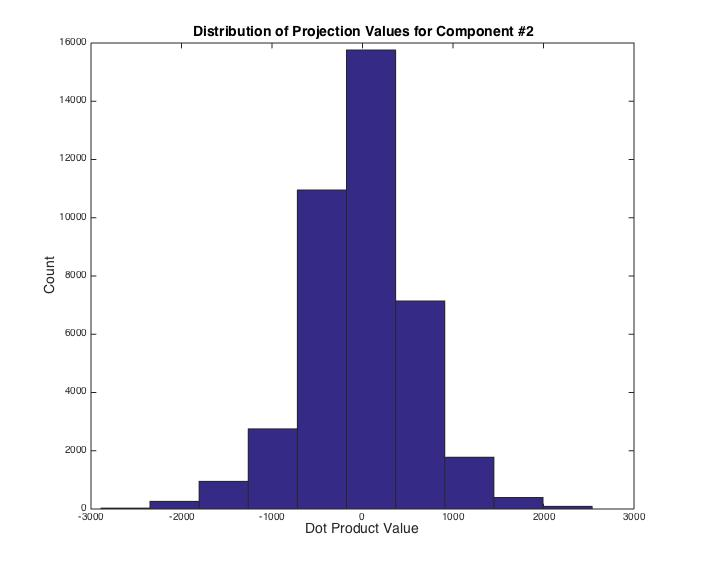
\includegraphics[width=1.0in]{fig_NN/hist_pp2.jpg}
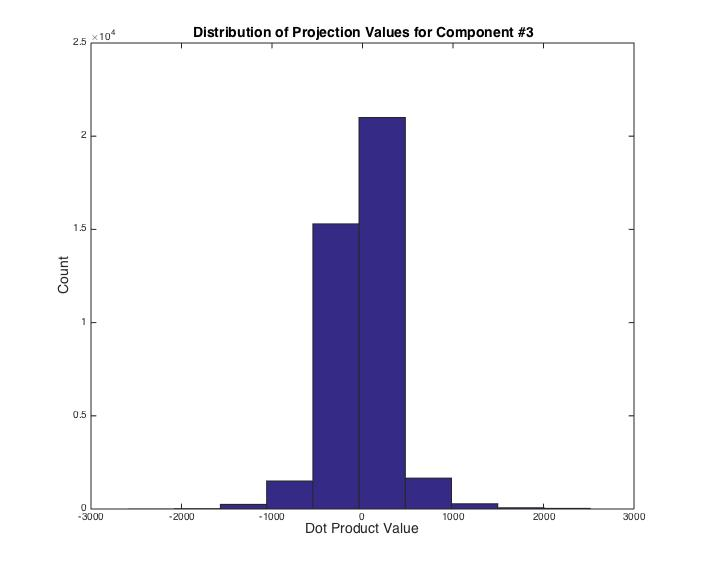
\includegraphics[width=1.0in]{fig_NN/hist_pp3.jpg}
\label{fig:pca-distr}
}
\caption{PCA-based hashing uses directions of maximal
variance in patches as projection vectors, and
adapt the bin size for each projection vector using data.
In b) we show distributions of patch vector projections
on the 3 principal components (magnitude of dot product).}
\label{fig:pca}
\end{figure}

To ensure that patches are well-distributed
among the bins, avoiding database lookup of many potential
neighbors, we propose a \emph{PCA-based hashing scheme}.
Under this scheme, we run Principal Component Analysis (PCA)
to compute directions of largest variance for typical image patches
and use 10 first principal components as the projection
directions (See Fig.~\ref{fig:pca}). This ensures that
the projections of typical patches are as far apart as possible.
To further optimize the binning, we project
a set of patches (grey dots in Fig.~\ref{fig:pca}) onto each
of principal component $\mathbf{v}_i$ (blue dots in Fig.~\ref{fig:pca}), and
approximate the distribution of the dot product
values by a Gaussian $\mathcal{N}_i(\mu_i, \sigma_i)$
(blue curve in Fig.~\ref{fig:pca}).
In order to bin a dot product value into one of 8 bins (3 bits/bin),
we adapt the bin size to $\mu_i$ and $\sigma_i$.

\begin{figure}[ht!]
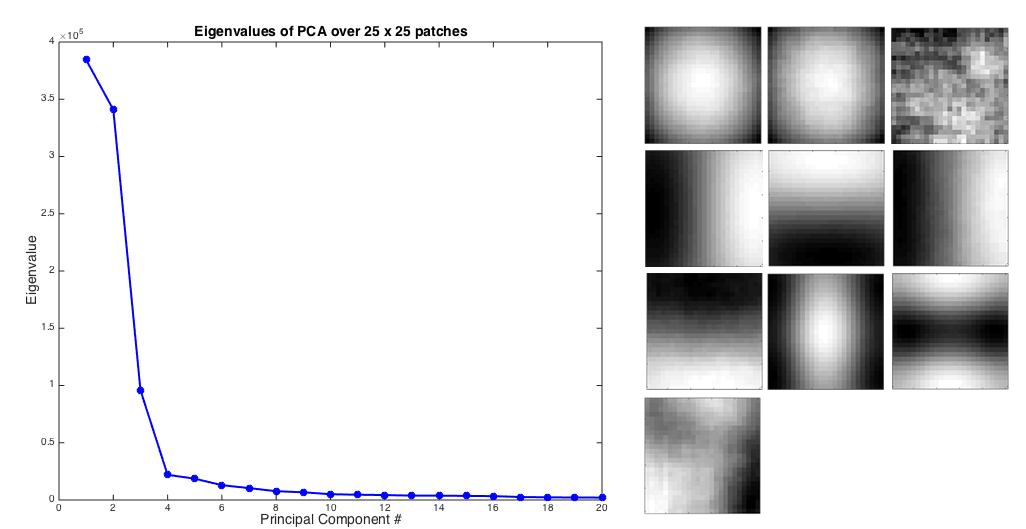
\includegraphics[width=3.0in]{fig_NN/principal_comps.png}
\caption{Eigenvalues of the PCA on 80K patches and visualization
of the L-channel (lightness) of the first 10 components.}
\label{fig:lambdas}
\end{figure}

In our experimental setup we sampled patches from two distinct
sets of 1000 images sampled uniformly from the SUN~\cite{SUN} database
(and distinct from the set of images we inserted into the database),
and used the patches to:
\begin{itemize}
\item compute PCA vectors in Luv color scheme on the \texttt{train{\allowbreak} set}
of 80,000 25x25 patches (See Fig.~\ref{fig:lambdas})
\item compute distribution of typical projections on 10
first principal components using the \texttt{dev{\allowbreak} set} of
40,000 25x25 patches (See Fig.~\ref{fig:pca-distr}).
\end{itemize}
We found that this choice of a hashing function has \emph{a
significant positive effect on performance}(See Sec.~\ref{sec:performance}).

\begin{figure}[ht!]
\subfigure[Pitfalls of standard deviation]{
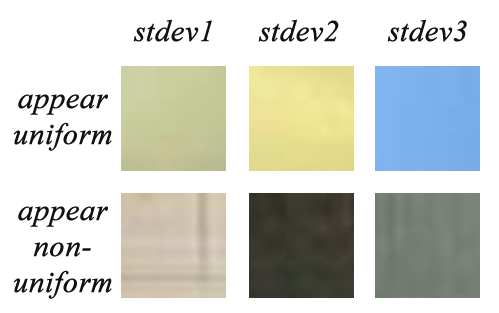
\includegraphics[width=2.5in]{fig_NN/std_uni.png}
\label{fig:color-stdev}}
\subfigure[Uniformity classification with p-norm]{
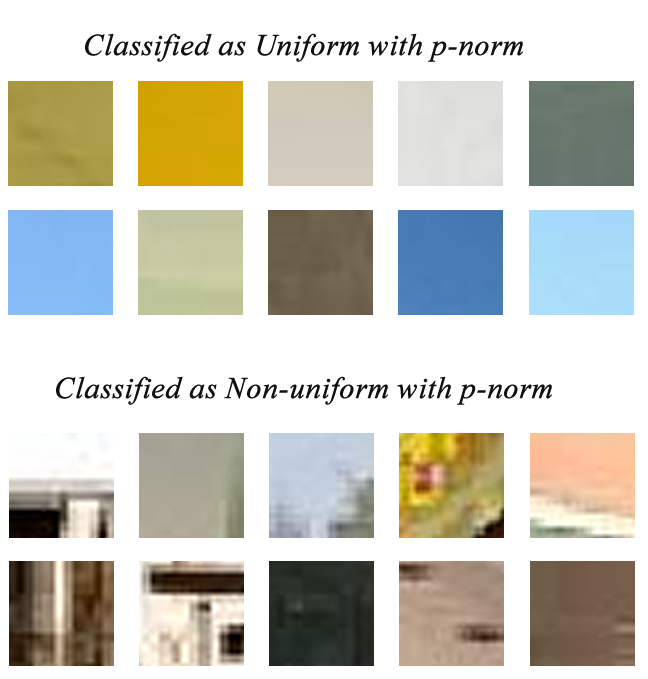
\includegraphics[width=3.0in]{fig_NN/uni_class.png}
\label{fig:color-pnorm}}
\caption{Standard deviation in a) is not very sensitive
to outliers, as patches with nearly identical
values of $stdev1$, $stdev2$ and $stdev3$ may appear
either uniform or non-uniform, as shown in the table.
In b), our classification of patches using
p-norm anecdotally shows more reliable results.}
\end{figure}

\subsection{Hashing Uniform Patches}\label{ssec:uni-nn}

The difficulty of Near Neighbor search for images arises from
their high dimensionality. However, natural images contain many uniform
or nearly uniform patches, which can be easily indexed using
their quantized color. We experimented with using a different
hashing scheme for patches that are nearly uniform, quantizing
them into fewer than 1000 bins by the mean color.

In order to determine if patch $P$ is uniformly colored, we first
looked at the standard deviation $u_2$ of the patch in all channels, which is
just the L-2 norm of $P-\mu(P)$, where $\mu{P}$ is a patch
with every pixel set to the mean of $P$.
However, we found that the L-2 norm is in-sensitive to outliers
(which are very apparent in color patches),
and patches with similar $u_2$ values could appear both uniform
and not-uniform (See Fig.~\ref{fig:color-stdev}).

Instead, we decided to classify uniformity using $u_4$, an L-4 norm
of $P-\mu(P)$, split into channels. Higher order forms tend
to collapse all values $< 1.0$ to zero, and expand all values $> 1.0$
to infinity. Hence, we normalize the elements of $P-\mu(P)$ by
our channel threshold $T$ to ensure this property. The best
approach would pick uniformity thresholds on $u_4$ using
a training set, but in the interests of time we hand-picked
a threshold of $0.1$ for all the channels. See Fig.~\ref{fig:color-pnorm}
for results of this classification on a random set of patches.

We evaluate the performance of PCA-based hashing compared to
a hybrid PCA+uniform patch hashing in Sec.~\ref{sec:performance}.


\subsection{DatabaseQueries}

We optimized our system to decrease database queries. In algorithm \ref{alg:insert}, for each image $I$ to insert, we have $\left(\frac{m}{n}\right)^2$ queries into the database to figure out whether there are patches that are similar to each of image's patches. Depending on whether there are similar patches in the database, we also make a query to insert a patch. This means for a single image insertion, we make $2\left(\frac{m}{n}\right)^2$ queries into the database (i.e. 2 queries per patch). This decreases the performance of our system. To solve this problem, we devised the following modified algorithm:

\begin{algorithm}
    \caption{Optimization of alg.~\ref{alg:insert2}, with ANN}
    \label{alg:optimized}
\begin{algorithmic}[1]
\State $Patches \leftarrow $ \texttt{Patchify}($I,n$)
\State $UniquePatches \leftarrow$ \texttt{FindUniquePatches}($I$)
\State $PatchesToStoreInDB \leftarrow []$
\For{$P_j$ in $UniquePatches$}
\State $SimPat \leftarrow $\texttt{FindLikelySimilarPatches}($P_j,patch\_dict$)
\State $P_{ANN} \leftarrow M(P_j)$
\If {$S(P_{ANN}, P_j) > T$}
\State {$PatchesToStoreInDB$.Add($P_j$)}
\EndIf
\EndFor
\State {\texttt{BatchInsert($PatchesToStoreInDB$)}}
\vspace{3mm}
\end{algorithmic}
\end{algorithm}

This batch insert ensures that for a single image, we at most query the database twice, once for finding all the likely similar patches in the database, and once to batch insert all the patches into the database. This reduces the queries made to the database by $\left(\frac{m}{n}\right)^2$ which is a significant improvement.
The idea of this algorithm is to do a local filtering among the patches of a single image before we query the database, such that the set of patches will only contain patches that are already greater than $T$ distance away from each other.  Let's call the filtered set the \emph{unique patches}. Then we query the database to find the set of likely to be similar patches to each of the unique patches. Only if none of the likely-to-be similar patches in the database matches a patch from the unique patches, do we insert this patch.

\section{Parameter Estimation}\label{sec:analysis}

A number of parameters can be tweaked to change the patch matching and storage, and different choices may be appropriate for different applications and performance requirements (both quantitative and qualitative). These parameters include the size of the input images, the size of the patches extracted, the sampling strategy used to seed the dictionary, the distance metric and thresholds used to compare patches, as well as the parameters required for indexing and retrieving patch matches (discussed in Sec.~\ref{sec:nn}). Here we discuss some of the parameter choices made and the experiments that lead up to these choices. Other possible choices are discussed in Sec.\ref{sec:futureext}.

Our quantitative performance metrics involve examining how the patch dictionary size grows with the addition of new images to the database (the growth function and rate) and the compression ratio per image (viewed as a distribution over compression ratios and summarized as the average compression ratio). Qualitative evaluations involve determining whether a human can spot compression artifacts and how salient they are in the images. The authors of this paper manually examined images reconstructed from the dictionary patches. A crowdsourced evaluation strategy would be more appropriate for larger-scale studies, but is beyond the scope of this paper.

There will always be a trade-off between compression benefits (storage: patch dictionary size and speed: image reconstruction time), and reconstruction quality. For many computer vision tasks including scene recognition (and thus retrieval), imperfect reconstructions with artifacts may not be a problem as long as the overall scene structure does not change. For instance, \cite{tiny_images} has shown that with images of pixel dimension 32x32, humans are already able to achieve over $80\%$ scene and object recognition rate. See fig.\ref{fig:badrecon} for a demonstration of an image that has serious reconstruction artifacts, but when downsampled to a thumbnail, they become insignificant, and thus may have no impact on visual recognition.

 \begin{figure}
%\hspace{-25mm}
\centering
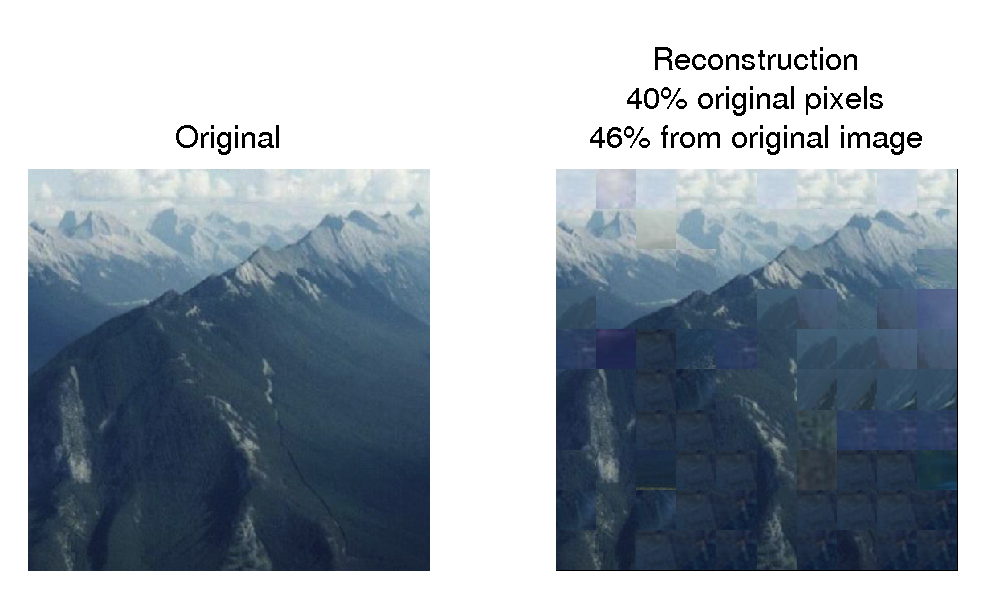
\includegraphics[width=0.7\linewidth]{Figures/184.png}
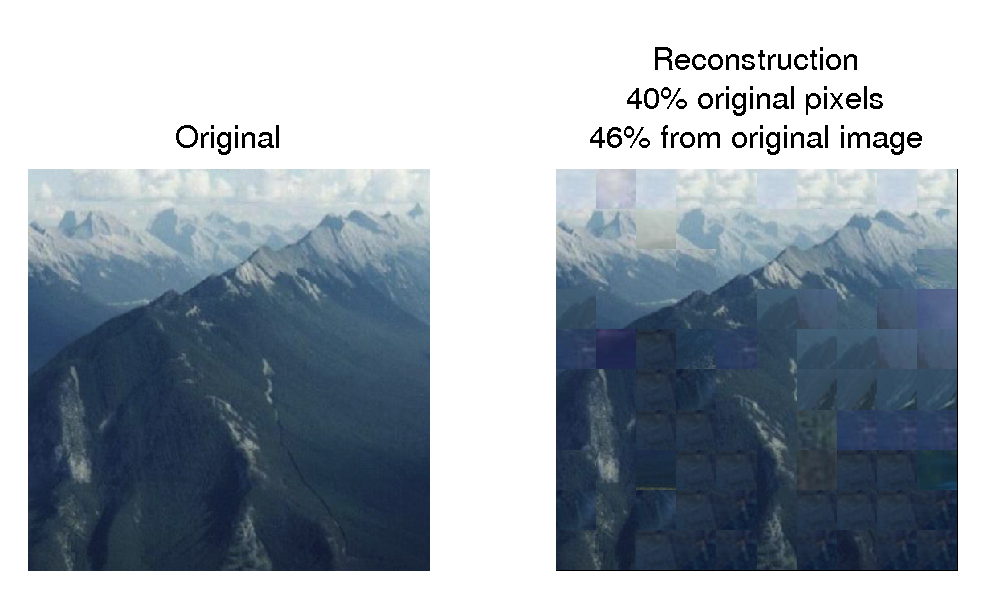
\includegraphics[width=0.3\linewidth]{Figures/184.png}
\caption{For demonstration purposes only, we choose a large patch size and low distance threshold. Under these parameters, the original image is reconstructed to take up only $40\%$ of its original size (in pixels). The $60\%$ of the patches that have been replaced come either from the same image ($46\%$ of them), or from other images (the remaining $64\%$). Notice that when the size of the image and its reconstruction are halved, the artifacts already become visually insignificant, and would not impair a scene recognition or search task. }
\label{fig:badrecon}
\end{figure}

 \begin{figure}
%\hspace{-25mm}
\centering
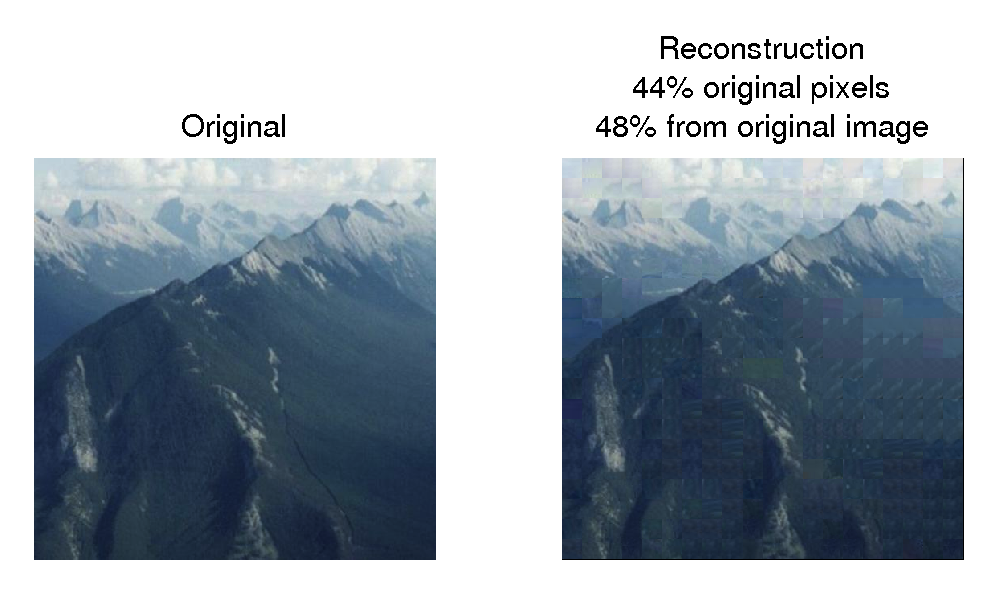
\includegraphics[width=0.7\linewidth]{Figures/184_25.png}
\caption{Compare this image reconstruction, computed with a dictionary of $25\times 25$ pixel patches with the reconstruction in fig.\ref{fig:badrecon}, computed with $50\times 50$ patches. In both cases, a similar threshold is used (scaled to the patch size, as discussed in sec. \ref{sec:simthresh}) but the visual artifacts are less noticeable because smaller patches have less contained structure, and are more likely to be homogenous in appearance.}
\label{fig:patchsize}
\end{figure}


%\subsection{Quality Metrics}\label{ssec:qual-met}
%There are many possible formulations of these quality constraints; we detail those that we considered for this paper in section TODO.  Beyond mathematical metrics, subjective methods are also interesting to consider for formulating the quality constraints; one could imagine a scenario in which image quality is assessed by humans through a crowdsourced system, perhaps using an engine such as Amazon's Mechanical Turk TODO: cite.  We consider such subjective similarity metrics outside the scope of this paper and focus on the mathematical metrics for now.

%We wish to construct a database that trades off minimizing the amount of required space with maximizing read and write speeds of the data.

\subsection{Patch Size}
\label{sec:patchsize}

%TODO(Zoya,Andrew): tradeoffs for patch size

%\begin{edit}
%(written by Andy): I think this should be moved earlier, after which the analysis is added.  Maybe we should add some stuff on the "quality gains" and add a plot for that, but there's not much we can probably do until later.
%\end{edit}

Larger patches contain more image structure, and thus the probability that another patch contains the same or similar image content decreases with the number of pixels in a patch. At larger granularities it becomes increasingly harder to find matching patches in the patch dictionary, and the closest matching patches for textured regions might introduce artifacts (see fig.\ref{fig:patchsize}). At the same time, patches that are too small do not offer as efficient a compression strategy. We must balance the costs of storing pointers to patches for each image in our database, as well as all the patches themselves, against the costs of storing the images in their original form. This calculation is investigated further below.

%In the extreme case, a patch is equal to one pixel, so the probability of an identical color patch is $\frac{1}{255^3}$, assuming 3 color channels. This value is multiplied by itself as many times as there are pixels in a patch to find an identical patch. For our application, we are interested in similar patches, rather than identical ones (see sec.\ref{sec:simthresh}), and so this probability is higher but bounded by this value, and similarly scales with patch size.

\subsubsection{Cost Evaluation}
\label{sec:costeval}

Assume, as before, that $d$ is the number of patches in \texttt{patch\_dict}.  In practice, $d$ is a function of the number of images added to the database as well as the distance function $S$ and threshold $T$.  We further assume that each pixel requires 3 bytes to store and that each pointer is 8 bytes (a standard integer for a 64-bit system).  Then, with $k$ images in the database, the full cost to store all the original images (no patch-based compression scheme) in our database is:

\begin{equation}
	 c'(k, m) = 3  k  m^2
\end{equation}

\noindent In the case where we store pointers to patches, we have two tables: one table to store pointers to dictionary patches, and a second table to store the dictionary patches themselves.  Under this ``patch pointer" scheme, with $k$ images and $d$ patches, the cost $c$ to store all the images in our database is:

\begin{equation}
	c(k, d, m, n) = 4 k \left(\frac{m}{n}\right)^2 + d (4 + 3 n^2)
\end{equation}.

The first term is the cost of storing the pointer data, while the second term is the cost of storing the patches themselves.  The $4$ constant comes from the fact that each pointer is a 4-bit int, while each patch requires storing $3$ color channels for $n^2$ pixels,
as well as a $4$ byte hash value.  Note that when dealing with extremely large image collections, it is possible to have over $2^{32}$ patches; in this case a \texttt{bigint} would be required for storing pointers, changing the $4$ to a $8$ and slightly changing the subsequent analysis.  In practice, we also store a bit more metadata to make managing the database easier, so this analysis should be thought of more as an optimal bound on storage.

Given these two equations, for a fixed $m$ and $n$, we can easily see that our compressive scheme becomes more space-efficient than storing the original images when:

\begin{equation}
	d < \frac{m^2 (3 - 4/(n^2)) k}{4 + 3n^2}
\end{equation}

As long as we choose a distance threshold such that new image patches get added at a rate that guarantees this inequality is satisfied, our compressive method of image storage will save space.  Figure \ref{fig:optcost} shows an example of how the optimal storage cost changes with different patch and image counts, where the optimal cost is defined as $c_{opt} = \min{(c, c')}$; in other words, storing the images using the less expensive method. See fig. \ref{fig:optcost}.

 \begin{figure}
%\hspace{-25mm}
%\centering
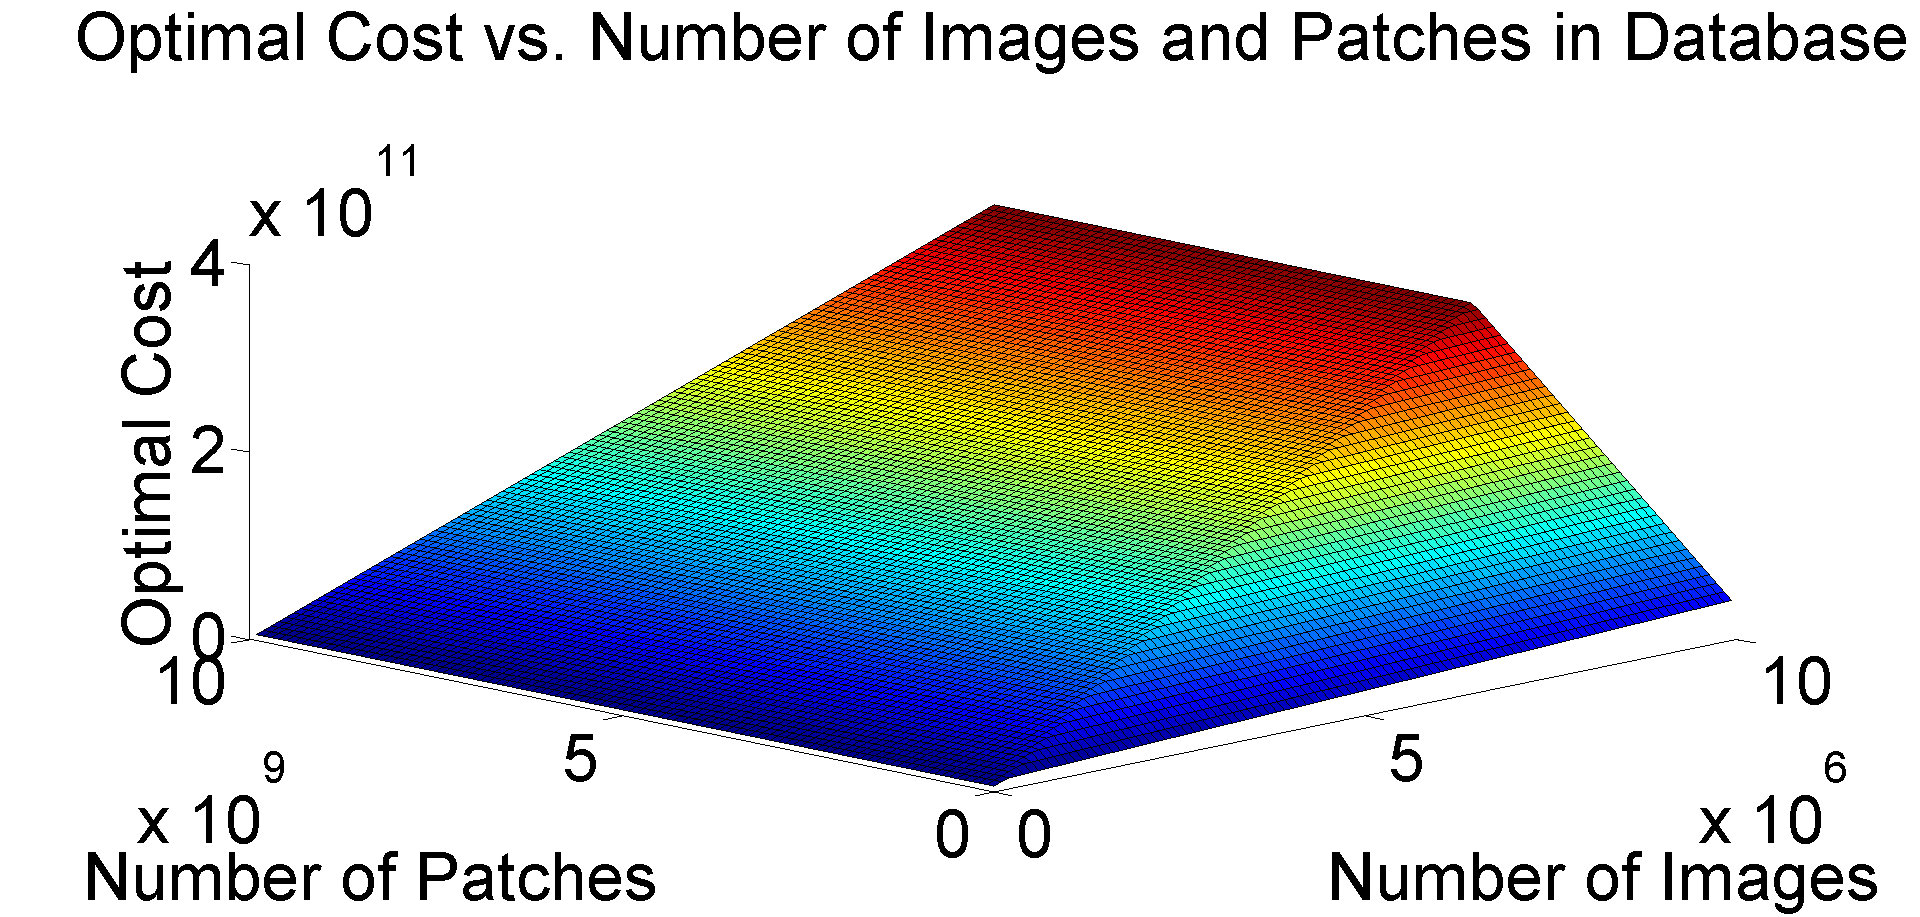
\includegraphics[width=1\linewidth]{Figures/PatchCosts.png}
\caption{A graph demonstrating how $c_{opt}$ changes with $k$ and $d$ for $m=100$ and $n=10$.  Note the line of discontinuity where $d = 357.3 k$ - this is the line where the costs of $c$ and $c'$ intersect.}
\label{fig:optcost}
\end{figure}


\subsection{Sampling strategies}
\label{sec:sample}

A patch dictionary can be built up incrementally, adding new patches as new images are added to the database. A potential problem with this approach is that image reconstruction quality will tend to decrease with the order in which images are added, such that images added to the database earlier will tend to have more patches that correspond to them (see Fig.\ref{fig:sampStrategy} for an example). A strategy with a more even distribution of reconstruction quality over images involves starting with a batch of images, and seeding the dictionary by randomly sampling patches from a set of images from the batch. This is the strategy we employ.

 \begin{figure}
%\hspace{-25mm}
\centering
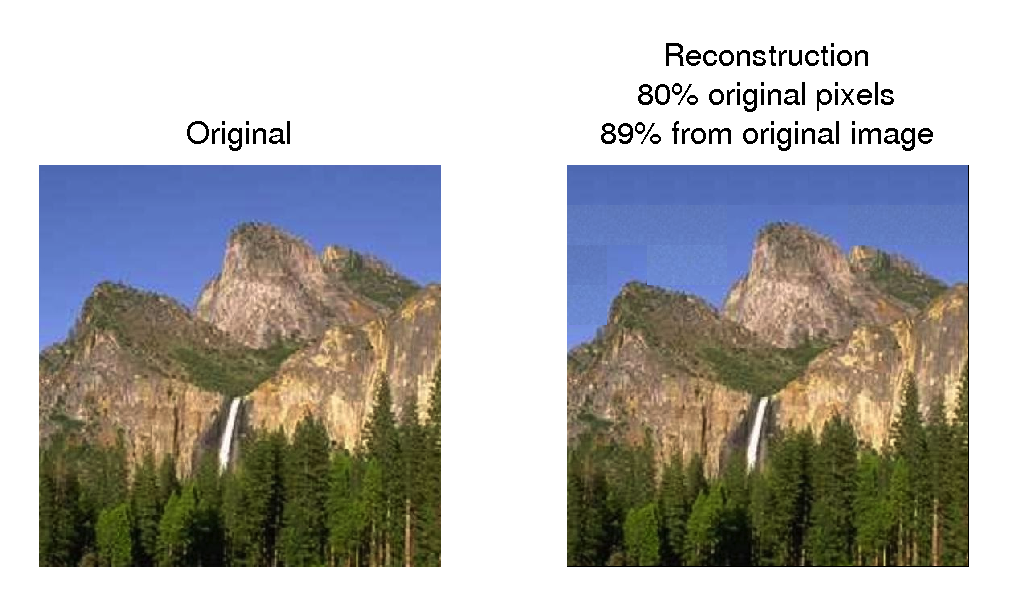
\includegraphics[width=0.7\linewidth]{Figures/009.png}
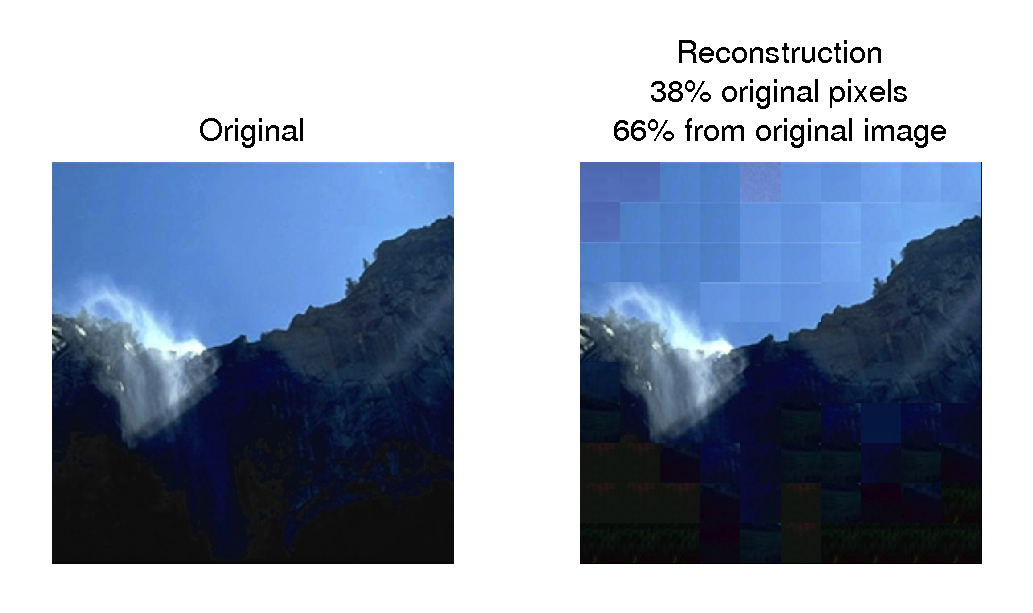
\includegraphics[width=0.7\linewidth]{Figures/014.png}
\caption{Example of a biased patch dictionary construction strategy, leading to non-uniformity in image reconstruction quality. Images added to the database earlier (top row) are better reconstructed (due to more patch samples in the database) than images added later (bottom row), constrained to be constructed out of patches added initially. The sky pixels in the image added later are borrowed from sky pixels of other images ($44\%$ of the pixels in this image come from other images, compared to only $11\%$ in the image on the first row). Note: here we use a very high patch distance threshold and large patch size for demonstration purposes only, to emphasize the artifacts created.}
\label{fig:sampStrategy}
\end{figure}


\subsection{Distance Function}
\label{sec:simthresh}

Many image (more specifically, patch) distance functions are possible, each with its own distinct set of parameters that can be tweaked for the required application. Because we are dealing with patches of a size specifically chosen to increase within-patch homogeneity, we do not consider cases of patches containing objects (the most we expect is an object boundary or simple texture), and thus do not need to consider complex image similarity/distance functions (involving SIFT, GIST, and other computer vision features). We can constrain ourselves to color distance, and split a patch $P_i$ into 3 LUV color channels: $P_i(L), P_i(U), P_i(V)$.

Then we consider two patches $P_i$ and $P_j$ similar when, given $n\times n$ pixels, all of the following are true:
\begin{align*}
\frac{1}{n^2}||P_i(L) - P_j(L)||^2 < T_1 \\
\frac{1}{n^2}||P_i(U) - P_j(U)||^2 < T_2 \\
\frac{1}{n^2}||P_i(V) - P_j(V)||^2 < T_3
\end{align*}

The $\frac{1}{n^2}$ term allows us to normalize for patch size, so that the threshold values chosen becomes independent of patch size. Here we constrain the average distance value of all the pixels in a patch to fit a threshold, whereas it is possible to have alternative constraints (where instead of the average, the maximal pixel difference or the variance of the pixel differences or some other measure over pixels in a patch, is compared to a threshold).

Note additionally that if instead we fix a single threshold for the sum of the Euclidean differences in the 3 color channels as in:
\begin{displaymath}
\frac{1}{n^2}[||P_i(L) - P_j(L)||^2 + ||P_i(U) - P_j(U)||^2 + ||P_i(V) - P_j(V)||^2] < T
\end{displaymath}
then the similarity in one color channel may compensate for the difference in another, producing skewed results (see fig.~\ref{fig:colProblem}).

Multiple color channels are possible, but we choose to work in the (CIE)LUV color space, which is known to be more perceptually uniform than the standard RGB color space~\cite{kekre2012performance}. Additionally, our formulation makes it possible to impose separate distance thresholds on each of the color channels ($T_1,T_2,T_3$). However, for simplicity of analysis, we set $T_1=T_2=T_3=T$, where the choice for the value of $T$ is described next.

\subsection{Distance Threshold}

Choosing a threshold $T$ requires weighing the quantitative benefits of compression with the qualitatively poorer image reconstructions. We ran a number of experiments, varying the threshold, and quantitatively and qualitatively examining the results. We rescale each color channel to be between 0 and 1, in order to choose a threshold $T$ that is bounded by these values. In fig.~\ref{fig:perfGraphs} we plot a few small experiments (with 200 images) for demonstrative purposes. The images were $500\times 500$ pixels, and the patch size was $25\times 25$. We chose this patch size due to the discussion in \ref{sec:patchsize}. Below we consider a number of quantitative indicators for patch compression.

In the set of graphs in the first column of fig.~\ref{fig:perfGraphs}, we plot in blue the dictionary size against the number of images added to the database. We compare this to the total number of patches that would have been stored if no compression scheme was utilized (red dotted line). We can see that for all choices of threshold, the size of the patch dictionary grows slower than the total number of patches that would need to be added if all images were stored along with their original patches. The gap between the blue and red dotted lines is a measure of the storage savings. As the threshold becomes more stringent, the blue line approaches the red dotted line. Note additionally that as the threshold becomes smaller, patches are more likely to be reused from the same image than from other images when compressing an image, because only patches from the same image will be similar enough to other patches from this image.

The second column of fig.~\ref{fig:perfGraphs} contains histograms indicating how many images contributed different amounts of new patches to the patch dictionary. When the threshold is very small (as in the histogram in the last row) more of the images contribute most of their patches (380-400 new patches added to the patch dictionary per image). Note additionally that the small number of images that are contributing 0 new patches to the dictionary account for the $10\%$ duplicates that are present in the SUN database (more about this in sec. \ref{sec:apps}).

The third column of fig. \ref{fig:perfGraphs} contains an insertion history: for each image inserted into the database, we track how many of its patches were added to the patch dictionary. We can see that as the patch distance threshold decreases, most images contribute most of their patches. This provides similar information as the histogram (which is merely the cumulative), but allows us to monitor any temporal changes. The spikes to 0 in this graph are indicative of duplicate images, and are discussed further in sec. \ref{sec:apps}.

In the final column of fig. \ref{fig:perfGraphs}, we see a sample image reconstruction. We can see that the reconstruction quality increases, and visual artifacts decrease, as the distance threshold decreases (becomes more stringent). At some point in the middle, the reconstruction is already indistinguishable from the original, but with significant database compression benefits. Thus, for further analysis we consider the threshold $T=0.01$ (recall that this is per color channel, and is independent of patch size).
%Thus, given two patches $P_i$ and $P_j$, we can measure their similarity in a given color channel by taking the Euclidean distance of the color values across all the pixels.

%where a patch is a collection of pixels, each of which is defined to be a triplet of integer values, assuming a 3-D color space. For a patch $P_i$, let us define its 3 color channels to be: $P_i(1), P_i(2), P_i(3)$.

 \begin{figure}
%\hspace{-25mm}
\centering
(a)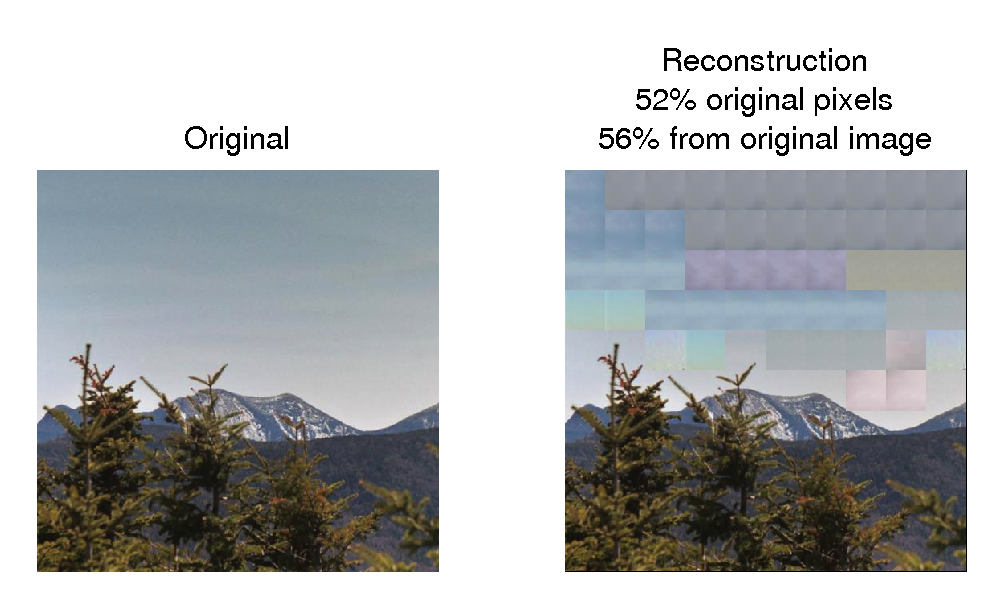
\includegraphics[width=0.7\linewidth]{Figures/197.png}
(b)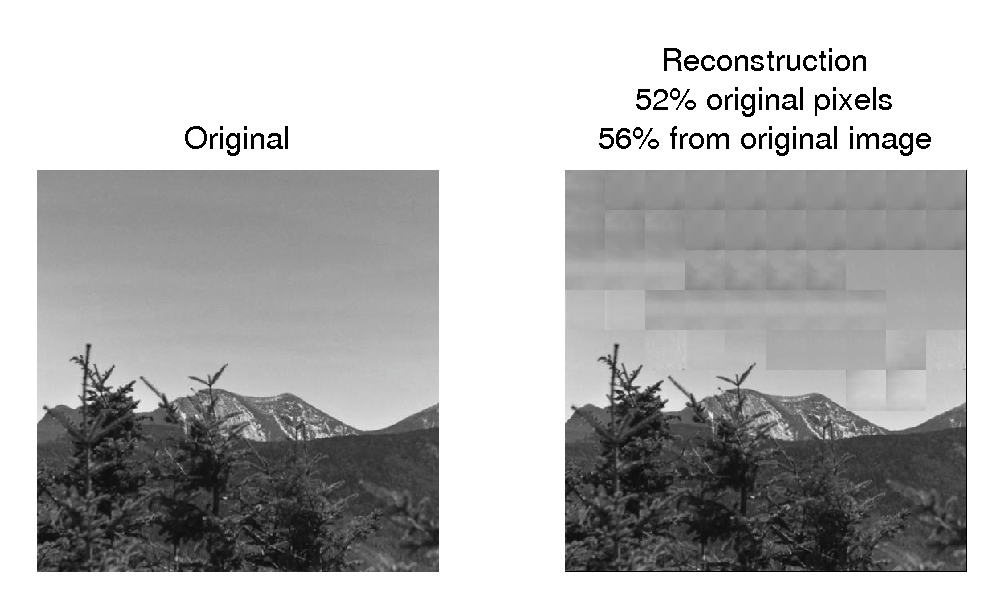
\includegraphics[width=0.7\linewidth]{Figures/197_bw.png}
\caption{This is what happens when we do not separately constrain each of the color channels to match. We have patches that are (a) the wrong color and produce visible visual artifacts, while (b) matching in terms of general hue (average of the color channels). Again, the patch size and distance threshold were chosen to emphasize the artifacts.}
\label{fig:colProblem}
\end{figure}

 \begin{figure*}
%\hspace{-25mm}
%\centering
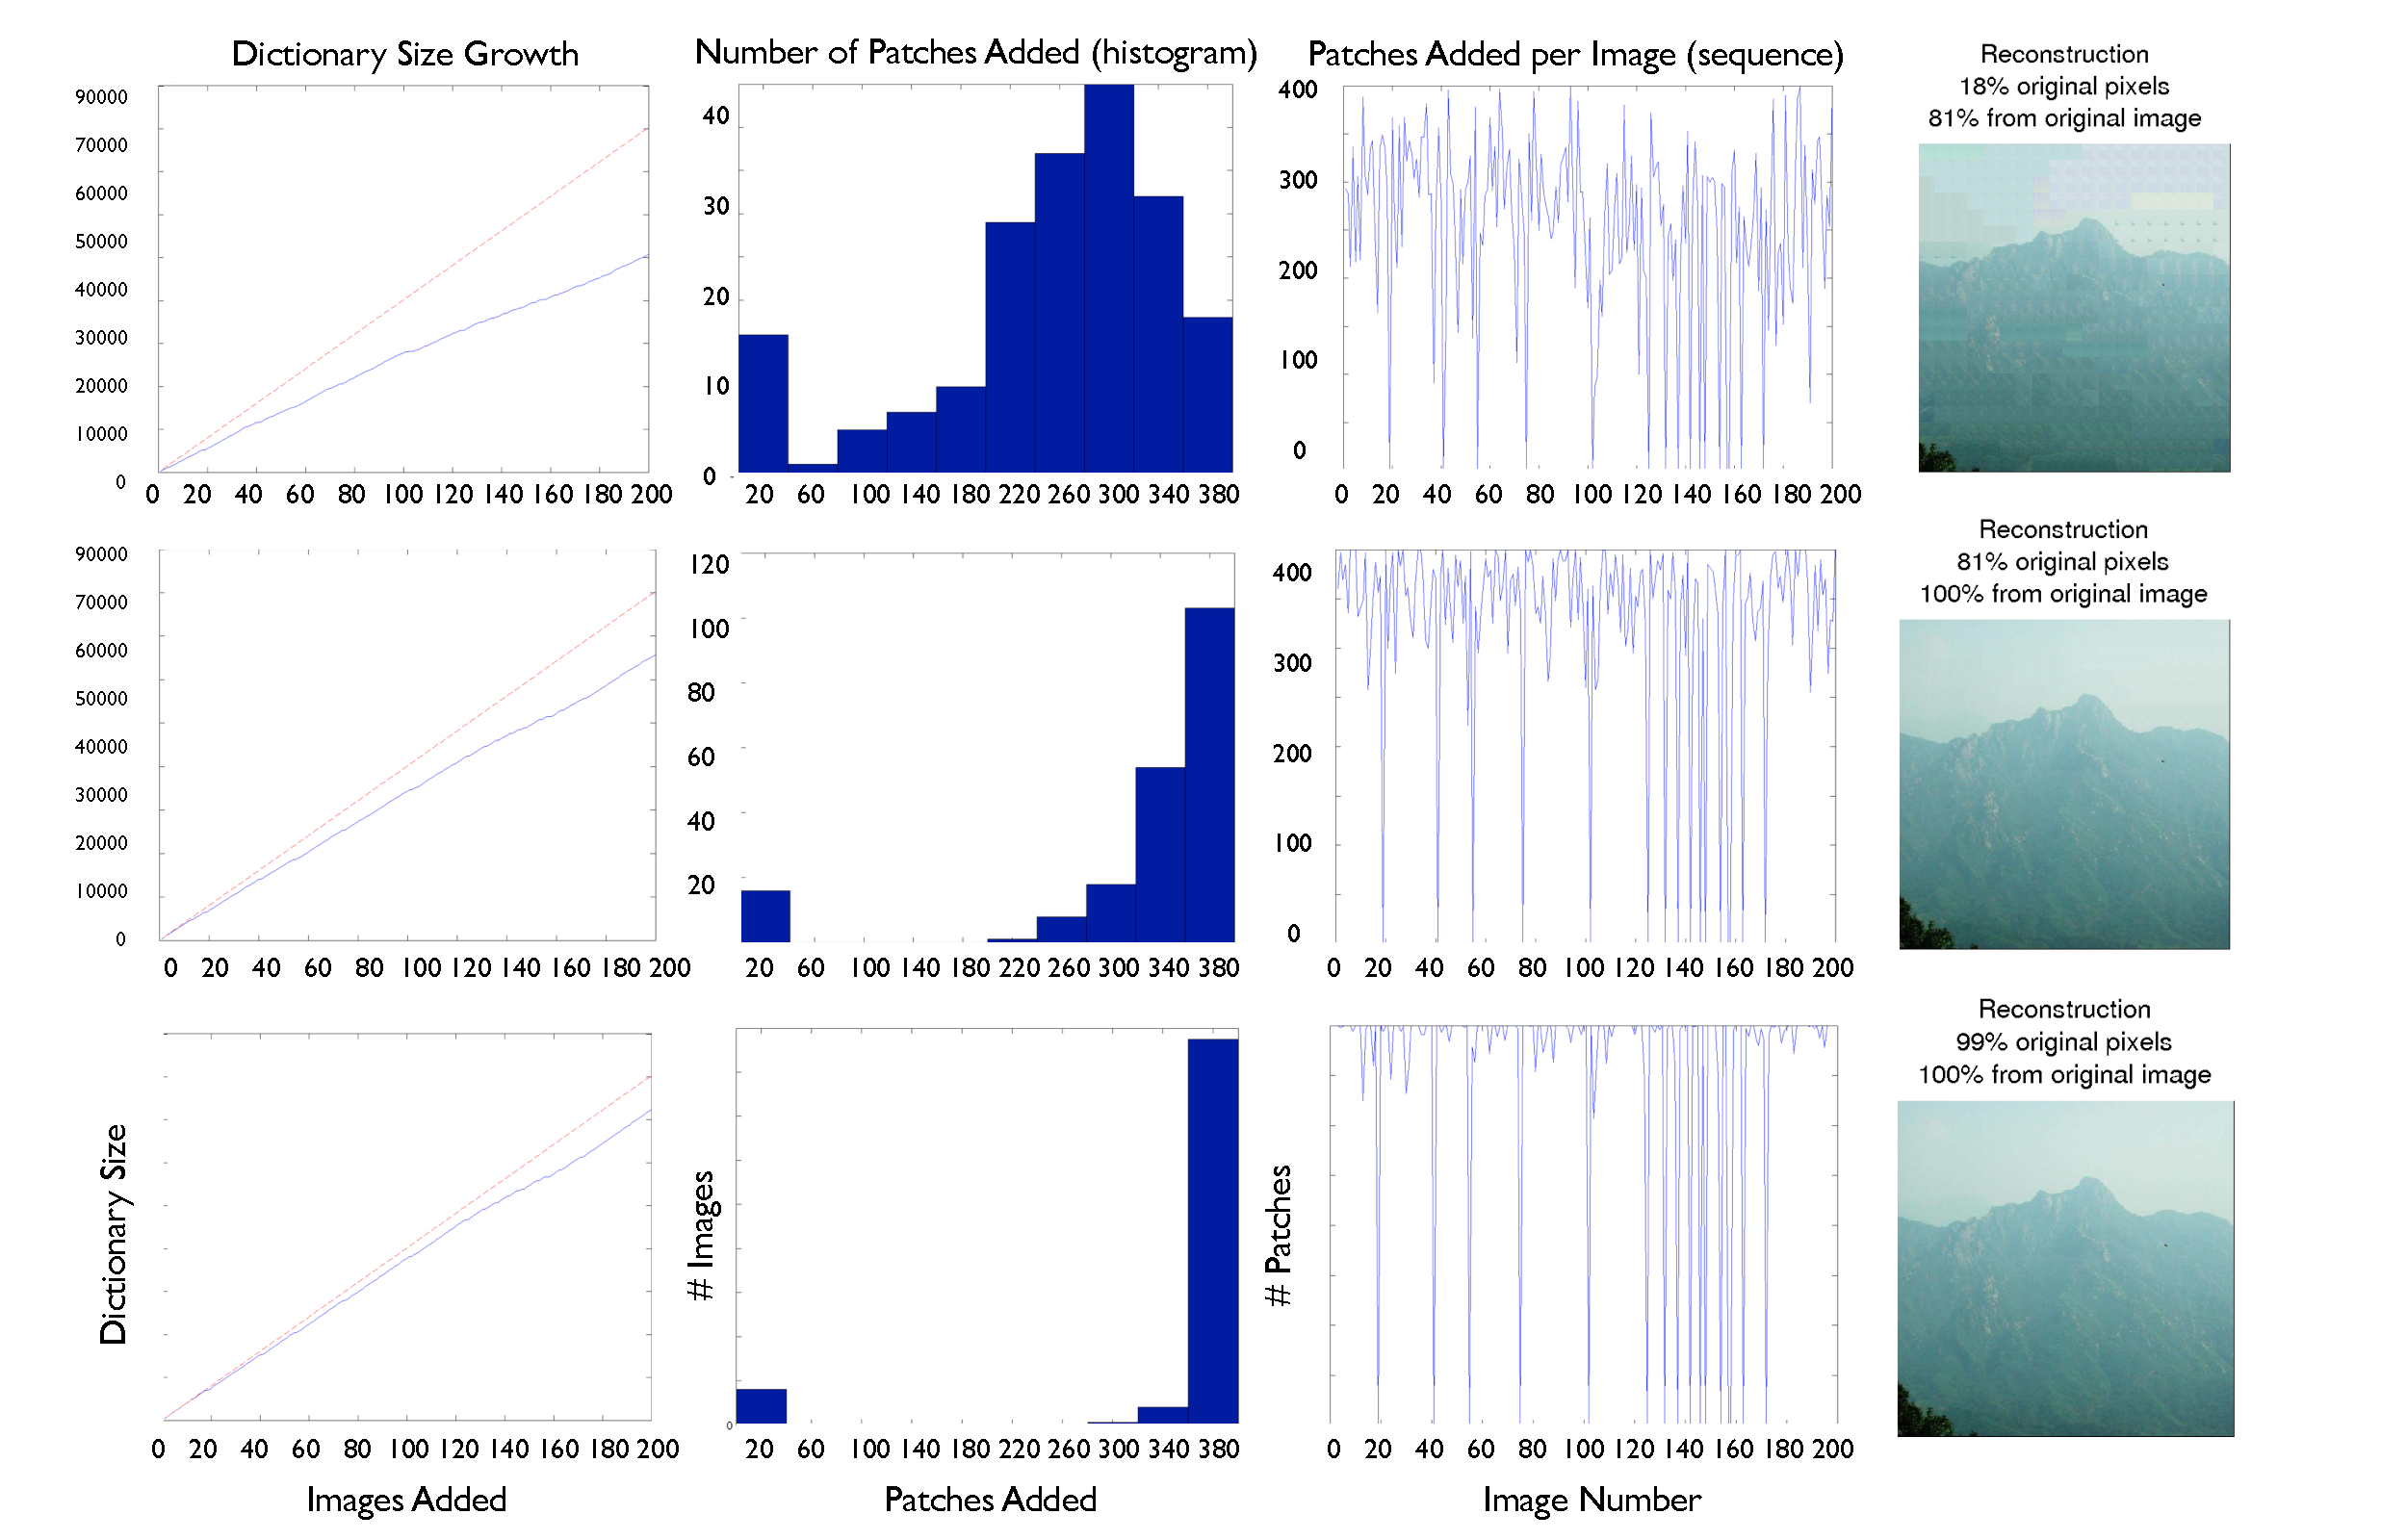
\includegraphics[width=1\linewidth]{Figures/perfGraphs_25_big.pdf}
\caption{Quantitative and qualitative results obtained by varying the patch distance threshold, $T$, while extracting $400$ patches from each image. In the first row, $T=0.1$, the dictionary size is 50,822 patches, and the average compression per image is $36.73\%$. In the second row, $T=0.01$, the dictionary size is $65,794$ patches, and the average compression per image is $18.09\%$. In the third row, $T=0.001$, the dictionary size is $72,445$ patches, and the average compression per image is $9.80\%$.}
\label{fig:perfGraphs}
\end{figure*}

\subsection{Generalization across image categories and sizes}
\label{sec:growing_db}

In the preceding sections, we determined that for an image sized $500\times 500$, a $25\times 25$ patch size with a $T=0.01$ patch distance threshold is appropriate since compression savings are properly balanced against artifacts introduced during image reconstruction. For further experiments, we scale down the image size to $100\times 100$ and the patch size to $5\times 5$, accordingly, maintaining the patch:image size ratio. Note that the distance threshold still applies as it is independent of patch size. The reduction in image size allows us to consider larger experiments on databases of image thumbnails.

In fig. \ref{fig:bigsize} we consider the growth of the patch dictionary as we add 2K images to our database. We add images from different categories, and observe a slight change in dictionary growth rate for every new category added. Although there is some variation across categories, the overall compression is $18.95\%$ per image, demonstrating generalization across categories.

 \begin{figure}
\hspace{-5mm}
%\centering
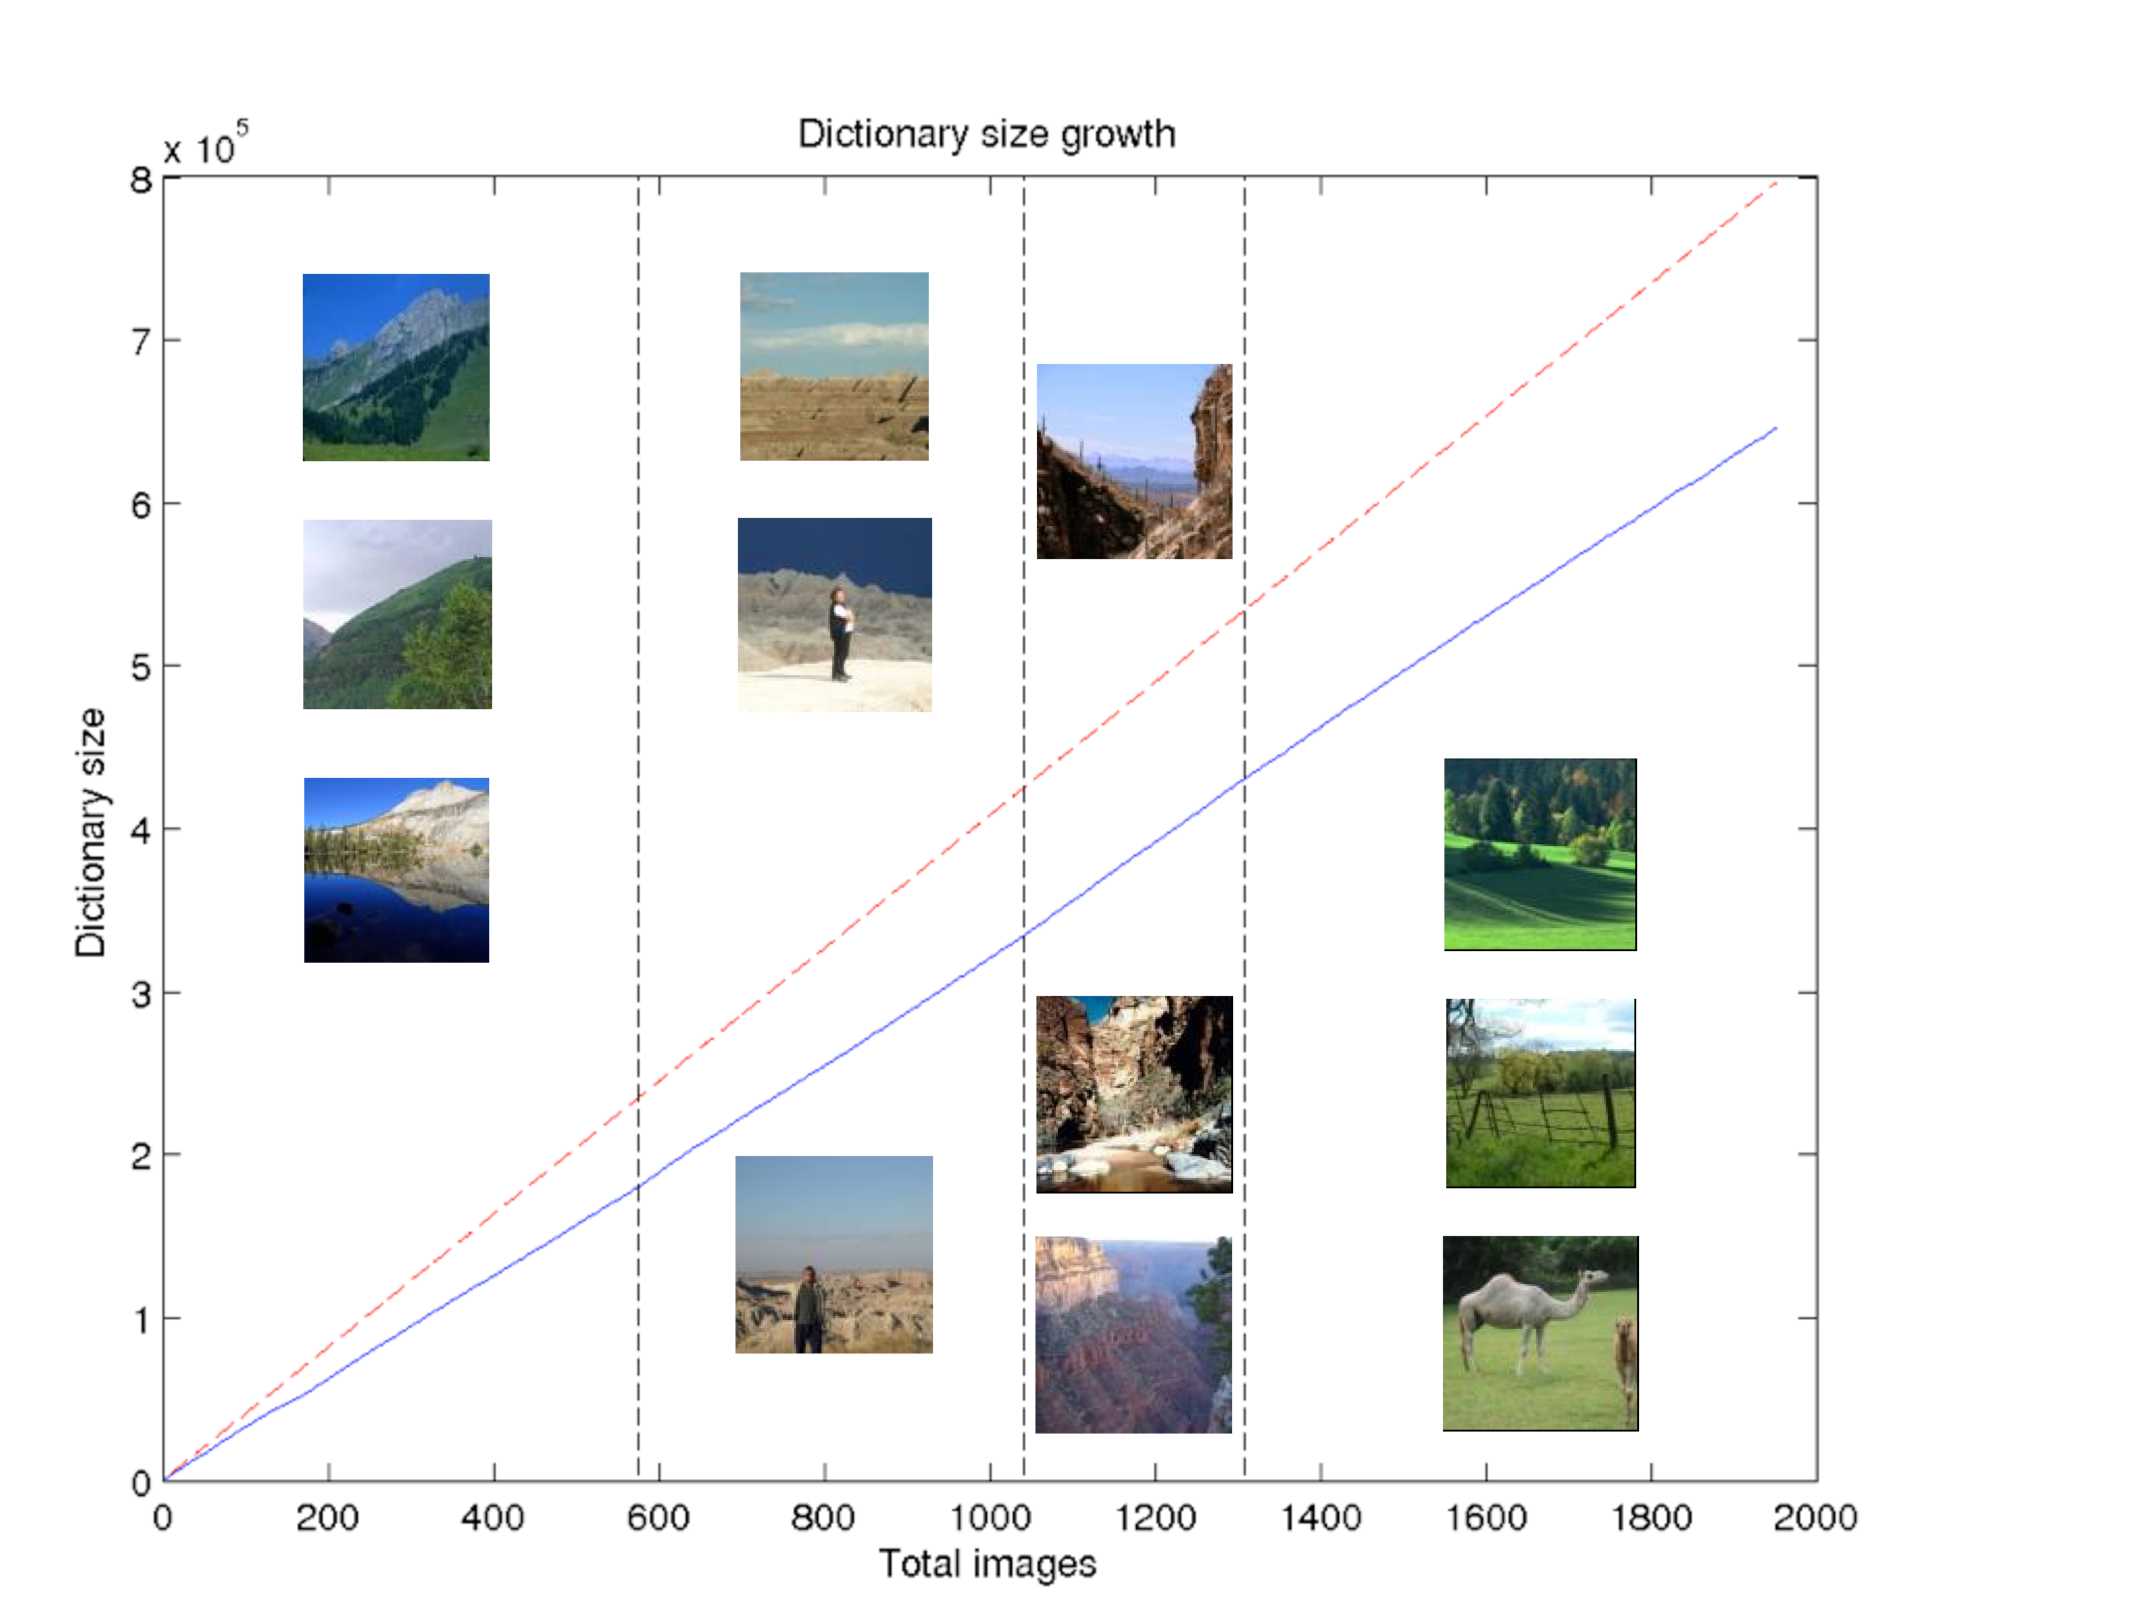
\includegraphics[width=1.3\linewidth]{Figures/multiscenes.pdf}
\caption{A patch dictionary constructed from $5\times 5$ patches from $100\times 100$ images, with a $T=0.01$ patch distance threshold, obtains an average compression of $18.95\%$ per image. The average number of new patches added per image is $330.70$ with a total dictionary size of $645,534$ patches representing 1952 images. The black dotted vertical lines mark the addition of new image categories, (left to right) mountain (with dictionary growth rate 312.96, equivalent to compression of $21.76\%$ per image), badlands (growth rate 330.50, compression $17.38\%$), canyon (growth rate: 360.61, compression $9.85\%$), and pasture (growth rate: 334.11, $16.47\%$). A few image samples from the 4 categories are included.  Note that for this growth rate, storing image patches will always take less space than storing the entire image, since $c < c'$.}
\label{fig:bigsize}
\end{figure}

Not all image content is amenable to the same type of compression. For some types of images, particularly where there is a lot of spatial structure (e.g. indoors scenes with objects and parts), compression artifacts are much more noticeable and thus distance thresholds should be more stringent. An interesting extension that is beyond the score of this paper would be to have a content-aware distance threshold (self-adjusting to content type such as indoor vs outdoor/natural).

For our database system, compression works for both indoor and outdoor images. In outdoor images, a lot of the compression savings come from accounting for the homogeneous sky patches (which may take up a large portion of the image). Although indoor images often contain many more objects and are more cluttered than outdoor images, they contain large homogenous regions corresponding to the walls and ceilings of rooms, which can surprisingly compress better than some outdoor images (walls may be more homogeneous than the sky). Thus, our compression approach generalizes to different types of scenes.

\section{Performance}\label{sec:performance}

In this section we evaluate the performance of our method
on a real collection of X images of Y size.

\subsection{Quantitative}\label{ssec:quant}


\subsection{Qualitative}\label{ssec:qual}

\section{Conclusion}

\begin{edit}
Summarize paper contributions
\end{edit}


\subsection{Applications}\label{sec:apps}

One of the appeals of this approximate patch-based approach
is that it naturally lends itself to applications. In this
section we describe methods to use our database for
two applications - duplicate detection and similar image retrieval.

\subsection{Duplicate Detection}\label{sec:dups}

Encoding images as pointers to a collection of patches provides the ability to quickly spot images that contain large overlapping regions (composed of the same patches). In the extreme case, if multiple images point to the same set of patches, then we know these images are duplicates. Duplicates are a big problem in big computer vision datasets because they occur frequently and are hard to manually remove. They occur frequently (sometimes up to $10\%$ of the time) because these datasets are automatically scraped from the internet, where the same image can occur under separate identifiers (on different websites, copied and uploaded by different users, etc.). The SUN database \cite{SUN} used in this paper is no exception.

Duplicates are difficult to detect because not all duplicates are pixel-wise identical: the same image encoded using different standards or sized to different dimensions (even when resized to the same dimension later) will look almost identical to the human eye, but will contain different pixel values. Our patch distance metric is forgiving to perturbation at the pixel-level as long as the patch is overall similar to another patch (see sec.\ref{sec:simthresh}). If multiple images map to the same set of patches that means that the corresponding patches in those images are within a distance threshold of each other (upper-bounded by $2T$). If multiple images map to all of the same patches, then we have good guarantees that the images are near-duplicates. Otherwise, the probability that every single patch matched would be low (i.e. low that two images are similar locally, for multiple local locations - as many locations as patches).

We can use these properties to spot duplicates in our database on-the-fly. For instance, when an image is added to the database, we can measure how many new patches the image contributed to the patch dictionary (because similar-enough patches could not be found), and how much of the image was mapped to pre-existing dictionary patches. When an image is reconstructed fully from the dictionary patches, and the patches it is reconstructed from all come from a single other image in the database, we know that the newly-added image is a duplicate. This is depicted in fig. \ref{fig:dups}.

By the same logic, similar images are those that overlap in terms of the patches they share in common. We can easily compare the two patch pointer vectors of two images to check their overlap. We can check if this overlap corresponds to patches clustered together in the images (for instance, when only some local region of the images matches, like when they share an object). We can thus discover images that have different degrees of overlap with other images.

 \begin{figure}
\hspace{-8mm}
%\centering
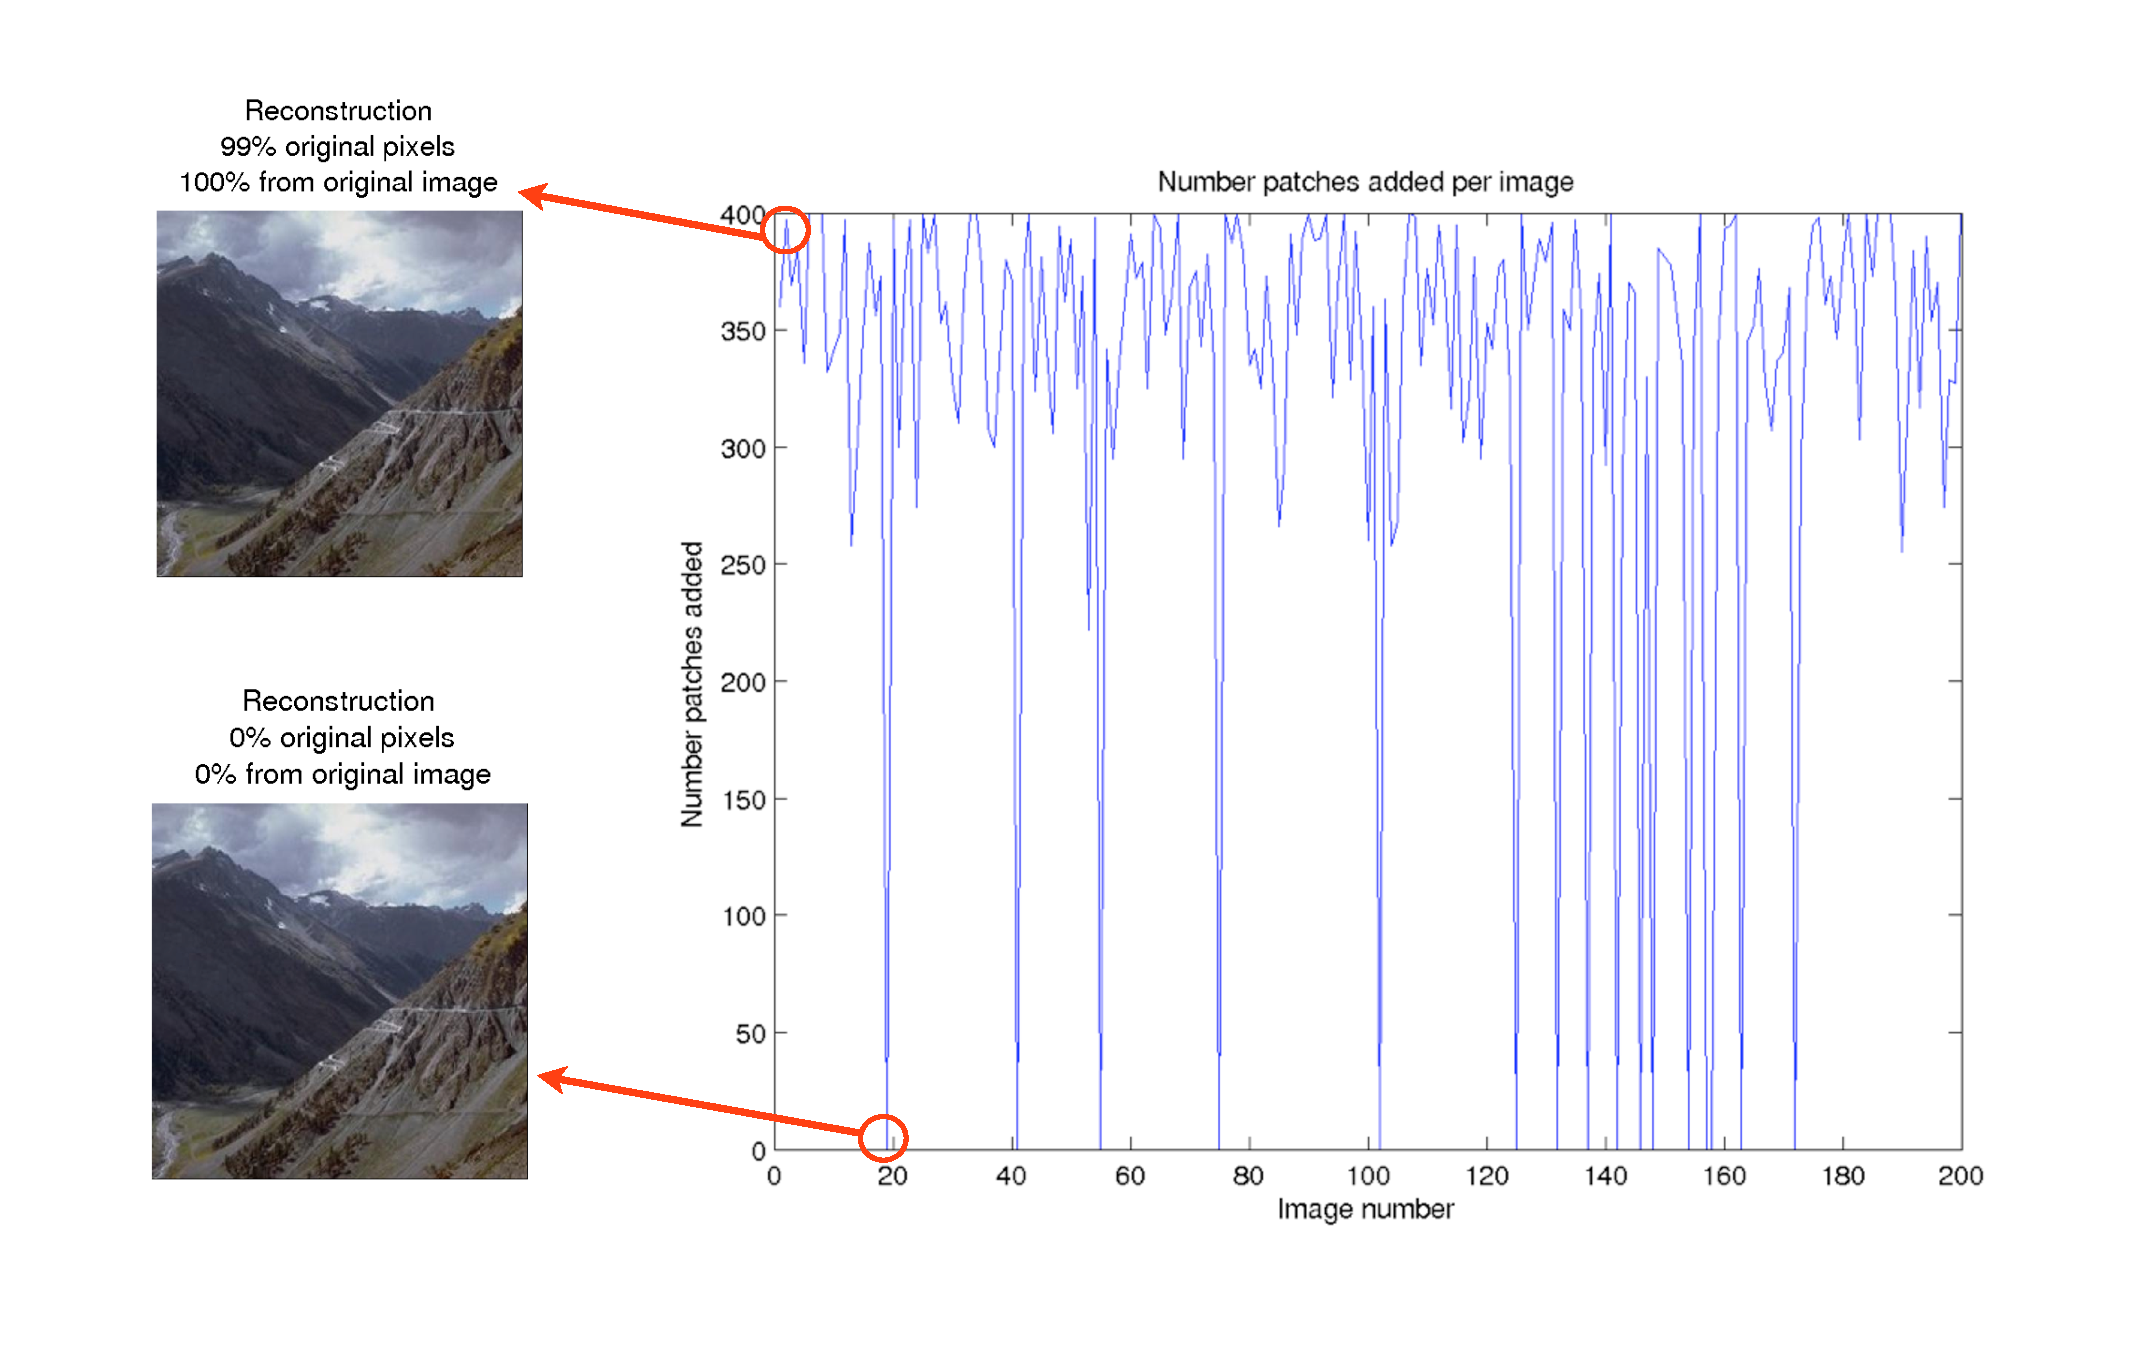
\includegraphics[width=1.2\linewidth]{Figures/dupDetection.pdf}
\caption{This is an example of the first 200 consecutive insertion queries to an empty database: for each image inserted, we can measure how many new patches were added to the patch dictionary (out of 400 patches in the image). When we see that this number spikes down to 0 we know that the image has been fully reconstructed from patches from other images. We can check if all those patches came from a single other image. If that is the case, we know we have a duplicate or near-duplicate image. }
\label{fig:dups}
\end{figure}

\subsection{Photomosaics}\label{sec:photo}

One interesting (and somewhat whimsical) application of our system is in the automated fabrication of photomosaics from images.  A photomosaic \footnote{See, for example, \url{http://en.wikipedia.org/wiki/Photographic_mosaic}.} is an image which is created by partitioning a pre-existing 2-D piece of artwork into small, equally sized rectangles each of which is then replaced with a small image which approximates the original color and texture of the rectangle, keeping the overall artwork recognizable.  Thus, the final result is an image composed of hundreds of smaller images.

Our system can be directly applied to the synthesis of such images, with a few very small modifications.  First, instead of determining which patches to store based on our previous dictionary and image collection, we a priori store a selected input image set as our patch dictionary, but scaled to "patch size."  For demonstration purposes, we created our patch dictionary by scaling down and storing the entire SUN database.  In order to create the photomosaic, we first choose and store a target image we would like to transform.  In storing the image, we, as usual split the image into patches, and for each patch perform a nearest neighbor search.  However, in this case, if no patch already exists in the hashed bin, we expand our nearest neighbor search to more bins until we find a bin with at least one patch, and choose the most similar one.  During this step, we \emph{never} store patches; we always map the patch to one already in the dictionary.  The mapping output by this process results in a photomosaic.

We demonstrate this process on a 1600x1200 image of the Stata Center at MIT, using 25x25 rectangular patches.  We show the original image and reconstruction in figure \ref{fig:stata}.





\subsection{Future Extensions}
\label{sec:futureext}

In this paper we considered a simple implementation of a patch-based image database compression scheme, where the images and patches were square and of fixed sizes. Patches were sampled in a regular, non-overlapping grid from each image.  Alternative approaches include more flexible, context-aware, patch-sampling techniques. For instance, the patch granularity for sampling large homogenous sky and field regions may be different from the one used for sampling highly-textured regions like objects and structures (trees, buildings, people, etc.). Similarly, patches that do not cross object boundaries are likely to lead to less artifacts in future reconstructions. For this, approaches like Selective Search \cite{UijlingsIJCV2013} that localize image regions likely to contain objects, may prove promising for sampling patches.

If patches were different sizes, then one of a number of extensions to the system would be required - for instance, (1) a patch transformation scheme, or (2) a hierarchical patch dictionary. A patch transformation scheme would permit each patch to be transformed (in a simple way - e.g. via rescaling) to match another patch with the same appearance but different (scale) parameters. For instance, a small patch in one image may be sufficient to account for a much larger part of another image, and rather than storing many separate patches of different sizes, we would benefit from quickly applying transformations to existing dictionary patches. To implement this system would require storing, for each image location, not only a pointer to a patch in the patch dictionary but also a transformation (e.g. a set of scaling parameters). Naturally, the cost function (to weigh the benefits of such a scheme vs storing the original images or even equally-sized patches) would need to take into account (a) the extra parameters stored along with each image location, and (b) the reconstruction time overhead for patch transformation. With large enough datasets, this approach may be effective at eliminating redundancy.

Another approach, building hierarchical patch dictionaries, may speed up the patchifying and subsequent reconstruction of an image, by offering a top-down approach. If larger patches match, there is no need to parse the image at a finer-grained scale. Only if large patches do not properly account for the structure in an image, would it be necessary to go to a finer-grained patch size. Note that small patches could be composed into larger patches, via a hierarchy, so that if large-patch matches are not found, descending down the patch hierarchy of the best-matching large patches would make it possible to find a match at a lower granularity. This scheme would be less flexible than the patch transformation scheme, but may prove to be more efficient. 



% NOTE: include this input to see all the latex tips
%\section{LATEX TIPS}

\subsection{Type Changes and {\subsecit Special} Characters}
We have already seen several typeface changes in this sample.  You
can indicate italicized words or phrases in your text with
the command \texttt{{\char'134}textit}; emboldening with the
command \texttt{{\char'134}textbf}
and typewriter-style (for instance, for computer code) with
\texttt{{\char'134}texttt}.  But remember, you do not
have to indicate typestyle changes when such changes are
part of the \textit{structural} elements of your
article; for instance, the heading of this subsection will
be in a sans serif\footnote{A third footnote, here.
Let's make this a rather short one to
see how it looks.} typeface, but that is handled by the
document class file. Take care with the use
of\footnote{A fourth, and last, footnote.}
the curly braces in typeface changes; they mark
the beginning and end of
the text that is to be in the different typeface.

You can use whatever symbols, accented characters, or
non-English characters you need anywhere in your document;
you can find a complete list of what is
available in the \textit{\LaTeX\
User's Guide}\cite{Lamport:LaTeX}.

\subsection{Math Equations}
You may want to display math equations in three distinct styles:
inline, numbered or non-numbered display.  Each of
the three are discussed in the next sections.

\subsubsection{Inline (In-text) Equations}
A formula that appears in the running text is called an
inline or in-text formula.  It is produced by the
\textbf{math} environment, which can be
invoked with the usual \texttt{{\char'134}begin. . .{\char'134}end}
construction or with the short form \texttt{\$. . .\$}. You
can use any of the symbols and structures,
from $\alpha$ to $\omega$, available in
\LaTeX\cite{Lamport:LaTeX}; this section will simply show a
few examples of in-text equations in context. Notice how
this equation: \begin{math}\lim_{n\rightarrow \infty}x=0\end{math},
set here in in-line math style, looks slightly different when
set in display style.  (See next section).

\subsubsection{Display Equations}
A numbered display equation -- one set off by vertical space
from the text and centered horizontally -- is produced
by the \textbf{equation} environment. An unnumbered display
equation is produced by the \textbf{displaymath} environment.

Again, in either environment, you can use any of the symbols
and structures available in \LaTeX; this section will just
give a couple of examples of display equations in context.
First, consider the equation, shown as an inline equation above:
\begin{equation}\lim_{n\rightarrow \infty}x=0\end{equation}
Notice how it is formatted somewhat differently in
the \textbf{displaymath}
environment.  Now, we'll enter an unnumbered equation:
\begin{displaymath}\sum_{i=0}^{\infty} x + 1\end{displaymath}
and follow it with another numbered equation:
\begin{equation}\sum_{i=0}^{\infty}x_i=\int_{0}^{\pi+2} f\end{equation}
just to demonstrate \LaTeX's able handling of numbering.

\subsection{Citations}
Citations to articles \cite{bowman:reasoning, clark:pct, braams:babel, herlihy:methodology},
conference
proceedings \cite{clark:pct} or books \cite{salas:calculus, Lamport:LaTeX} listed
in the Bibliography section of your
article will occur throughout the text of your article.
You should use BibTeX to automatically produce this bibliography;
you simply need to insert one of several citation commands with
a key of the item cited in the proper location in
the \texttt{.tex} file \cite{Lamport:LaTeX}.
The key is a short reference you invent to uniquely
identify each work; in this sample document, the key is
the first author's surname and a
word from the title.  This identifying key is included
with each item in the \texttt{.bib} file for your article.

The details of the construction of the \texttt{.bib} file
are beyond the scope of this sample document, but more
information can be found in the \textit{Author's Guide},
and exhaustive details in the \textit{\LaTeX\ User's
Guide}\cite{Lamport:LaTeX}.

This article shows only the plainest form
of the citation command, using \texttt{{\char'134}cite}.
This is what is stipulated in the SIGS style specifications.
No other citation format is endorsed.

\subsection{Tables}
Because tables cannot be split across pages, the best
placement for them is typically the top of the page
nearest their initial cite.  To
ensure this proper ``floating'' placement of tables, use the
environment \textbf{table} to enclose the table's contents and
the table caption.  The contents of the table itself must go
in the \textbf{tabular} environment, to
be aligned properly in rows and columns, with the desired
horizontal and vertical rules.  Again, detailed instructions
on \textbf{tabular} material
is found in the \textit{\LaTeX\ User's Guide}.

Immediately following this sentence is the point at which
Table 1 is included in the input file; compare the
placement of the table here with the table in the printed
dvi output of this document.

\begin{table}
\centering
\caption{Frequency of Special Characters}
\begin{tabular}{|c|c|l|} \hline
Non-English or Math&Frequency&Comments\\ \hline
\O & 1 in 1,000& For Swedish names\\ \hline
$\pi$ & 1 in 5& Common in math\\ \hline
\$ & 4 in 5 & Used in business\\ \hline
$\Psi^2_1$ & 1 in 40,000& Unexplained usage\\
\hline\end{tabular}
\end{table}

To set a wider table, which takes up the whole width of
the page's live area, use the environment
\textbf{table*} to enclose the table's contents and
the table caption.  As with a single-column table, this wide
table will ``float" to a location deemed more desirable.
Immediately following this sentence is the point at which
Table 2 is included in the input file; again, it is
instructive to compare the placement of the
table here with the table in the printed dvi
output of this document.


\begin{table*}
\centering
\caption{Some Typical Commands}
\begin{tabular}{|c|c|l|} \hline
Command&A Number&Comments\\ \hline
\texttt{{\char'134}alignauthor} & 100& Author alignment\\ \hline
\texttt{{\char'134}numberofauthors}& 200& Author enumeration\\ \hline
\texttt{{\char'134}table}& 300 & For tables\\ \hline
\texttt{{\char'134}table*}& 400& For wider tables\\ \hline\end{tabular}
\end{table*}
% end the environment with {table*}, NOTE not {table}!

\subsection{Figures}
Like tables, figures cannot be split across pages; the
best placement for them
is typically the top or the bottom of the page nearest
their initial cite.  To ensure this proper ``floating'' placement
of figures, use the environment
\textbf{figure} to enclose the figure and its caption.

This sample document contains examples of \textbf{.pdf} files to be
displayable with \LaTeX (See Figures \ref{fig:fly} and \ref{fig:bigfly}).  More details on each of these is found in the
\textit{Author's Guide}.

\begin{figure}
\centering
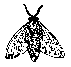
\includegraphics{fly.pdf}
\caption{A sample black and white graphic (.pdf format).}
\label{fig:fly}
\end{figure}

\begin{figure}
\centering
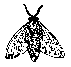
\includegraphics[width=1in,height=1in]{fly.pdf}
\caption{A sample black and white graphic (.pdf format)
that has been resized with the \texttt{includegraphics} command.}
\label{fig:bigfly}
\end{figure}


As was the case with tables, you may want a figure
that spans two columns.  To do this, and still to
ensure proper ``floating'' placement of tables, use the environment
\textbf{figure*} to enclose the figure and its caption (See Figure~\ref{fig:flies}). And don't forget to end the environment with {figure*}, not {figure}!

\begin{figure*}
\centering
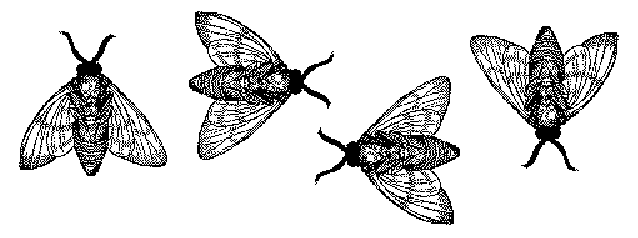
\includegraphics{flies}
\caption{A sample black and white graphic (.pdf format)
that needs to span two columns of text.}
\label{fig:flies}
\end{figure*}


Note that only {\textbf{.pdf}} files were used; if you want to include
{\textbf{.ps}} or {\textbf{.eps}} formats, you can use the
\texttt{{\char'134}epsfig} or \texttt{{\char'134}psfig}
commands as appropriate for the different file types.

\subsection{Theorem-like Constructs}
Other common constructs that may occur in your article are
the forms for logical constructs like theorems, axioms,
corollaries and proofs.  There are
two forms, one produced by the
command \texttt{{\char'134}newtheorem} and the
other by the command \texttt{{\char'134}newdef}; perhaps
the clearest and easiest way to distinguish them is
to compare the two in the output of this sample document:

This uses the \textbf{theorem} environment, created by
the\linebreak\texttt{{\char'134}newtheorem} command:
\newtheorem{theorem}{Theorem}
\begin{theorem}
Let $f$ be continuous on $[a,b]$.  If $G$ is
an antiderivative for $f$ on $[a,b]$, then
\begin{displaymath}\int^b_af(t)dt = G(b) - G(a).\end{displaymath}
\end{theorem}

The other uses the \textbf{definition} environment, created
by the \texttt{{\char'134}newdef} command:
\newdef{definition}{Definition}
\begin{definition}
If $z$ is irrational, then by $e^z$ we mean the
unique number which has
logarithm $z$: \begin{displaymath}{\log e^z = z}\end{displaymath}
\end{definition}

Two lists of constructs that use one of these
forms is given in the
\textit{Author's  Guidelines}.


There is one other similar construct environment, which is
already set up
for you; i.e. you must \textit{not} use
a \texttt{{\char'134}newdef} command to
create it: the \textbf{proof} environment.  Here
is a example of its use:
\begin{proof}
Suppose on the contrary there exists a real number $L$ such that
\begin{displaymath}
\lim_{x\rightarrow\infty} \frac{f(x)}{g(x)} = L.
\end{displaymath}
Then
\begin{align*}
l&=\lim_{x\rightarrow c} f(x)
= \lim_{x\rightarrow c}
\left[ g{x} \cdot \frac{f(x)}{g(x)} \right ] \\
&= \lim_{x\rightarrow c} g(x) \cdot \lim_{x\rightarrow c}
\frac{f(x)}{g(x)} = 0\cdot L = 0,
\end{align*}
which contradicts our assumption that $l\neq 0$.
\end{proof}

Complete rules about using these environments and using the
two different creation commands are in the
\textit{Author's Guide}; please consult it for more
detailed instructions.  If you need to use another construct,
not listed therein, which you want to have the same
formatting as the Theorem
or the Definition\cite{salas:calculus} shown above,
use the \texttt{{\char'134}newtheorem} or the
\texttt{{\char'134}newdef} command,
respectively, to create it.

\subsection*{A {\secit Caveat} for the \TeX\ Expert}
Because you have just been given permission to
use the \texttt{{\char'134}newdef} command to create a
new form, you might think you can
use \TeX's \texttt{{\char'134}def} to create a
new command: \textit{Please refrain from doing this!}
Remember that your \LaTeX\ source code is primarily intended
to create camera-ready copy, but may be converted
to other forms -- e.g. HTML. If you inadvertently omit
some or all of the \texttt{{\char'134}def}s recompilation will
be, to say the least, problematic.

\section{Conclusions}
This paragraph will end the body of this sample document.
Remember that you might still have Acknowledgments or
Appendices; brief samples of these
follow.  There is still the Bibliography to deal with; and
we will make a disclaimer about that here: with the exception
of the reference to the \LaTeX\ book, the citations in
this paper are to articles which have nothing to
do with the present subject and are used as
examples only.
%\end{document}  % This is where a 'short' article might terminate

% ensure same length columns on last page (might need two sub-sequent latex runs)
\balance

%ACKNOWLEDGMENTS are optional
\section{Acknowledgments}
This section is optional; it is a location for you
to acknowledge grants, funding, editing assistance and
what have you.  In the present case, for example, the
authors would like to thank Gerald Murray of ACM for
his help in codifying this \textit{Author's Guide}
and the \textbf{.cls} and \textbf{.tex} files that it describes.


% The following two commands are all you need in the
% initial runs of your .tex file to
% produce the bibliography for the citations in your paper.
%\bibliographystyle{abbrv}
%\bibliography{vldb_sample}  % vldb_sample.bib is the name of the Bibliography in this case
% You must have a proper ".bib" file
%  and remember to run:
% latex bibtex latex latex
% to resolve all references

\subsection{References}
Generated by bibtex from your ~.bib file.  Run latex,
then bibtex, then latex twice (to resolve references).

%APPENDIX is optional.
% ****************** APPENDIX **************************************
% Example of an appendix; typically would start on a new page
%pagebreak

\begin{appendix}
You can use an appendix for optional proofs or details of your evaluation which are not absolutely necessary to the core understanding of your paper.

\section{Final Thoughts on Good Layout}
Please use readable font sizes in the figures and graphs. Avoid tempering with the correct border values, and the spacing (and format) of both text and captions of the PVLDB format (e.g. captions are bold).

At the end, please check for an overall pleasant layout, e.g. by ensuring a readable and logical positioning of any floating figures and tables. Please also check for any line overflows, which are only allowed in extraordinary circumstances (such as wide formulas or URLs where a line wrap would be counterintuitive).

Use the \texttt{balance} package together with a \texttt{\char'134 balance} command at the end of your document to ensure that the last page has balanced (i.e. same length) columns.
\end{appendix}


\bibliographystyle{abbrv}
\bibliography{db_report}

\clearpage
 \begin{figure*}
\centering
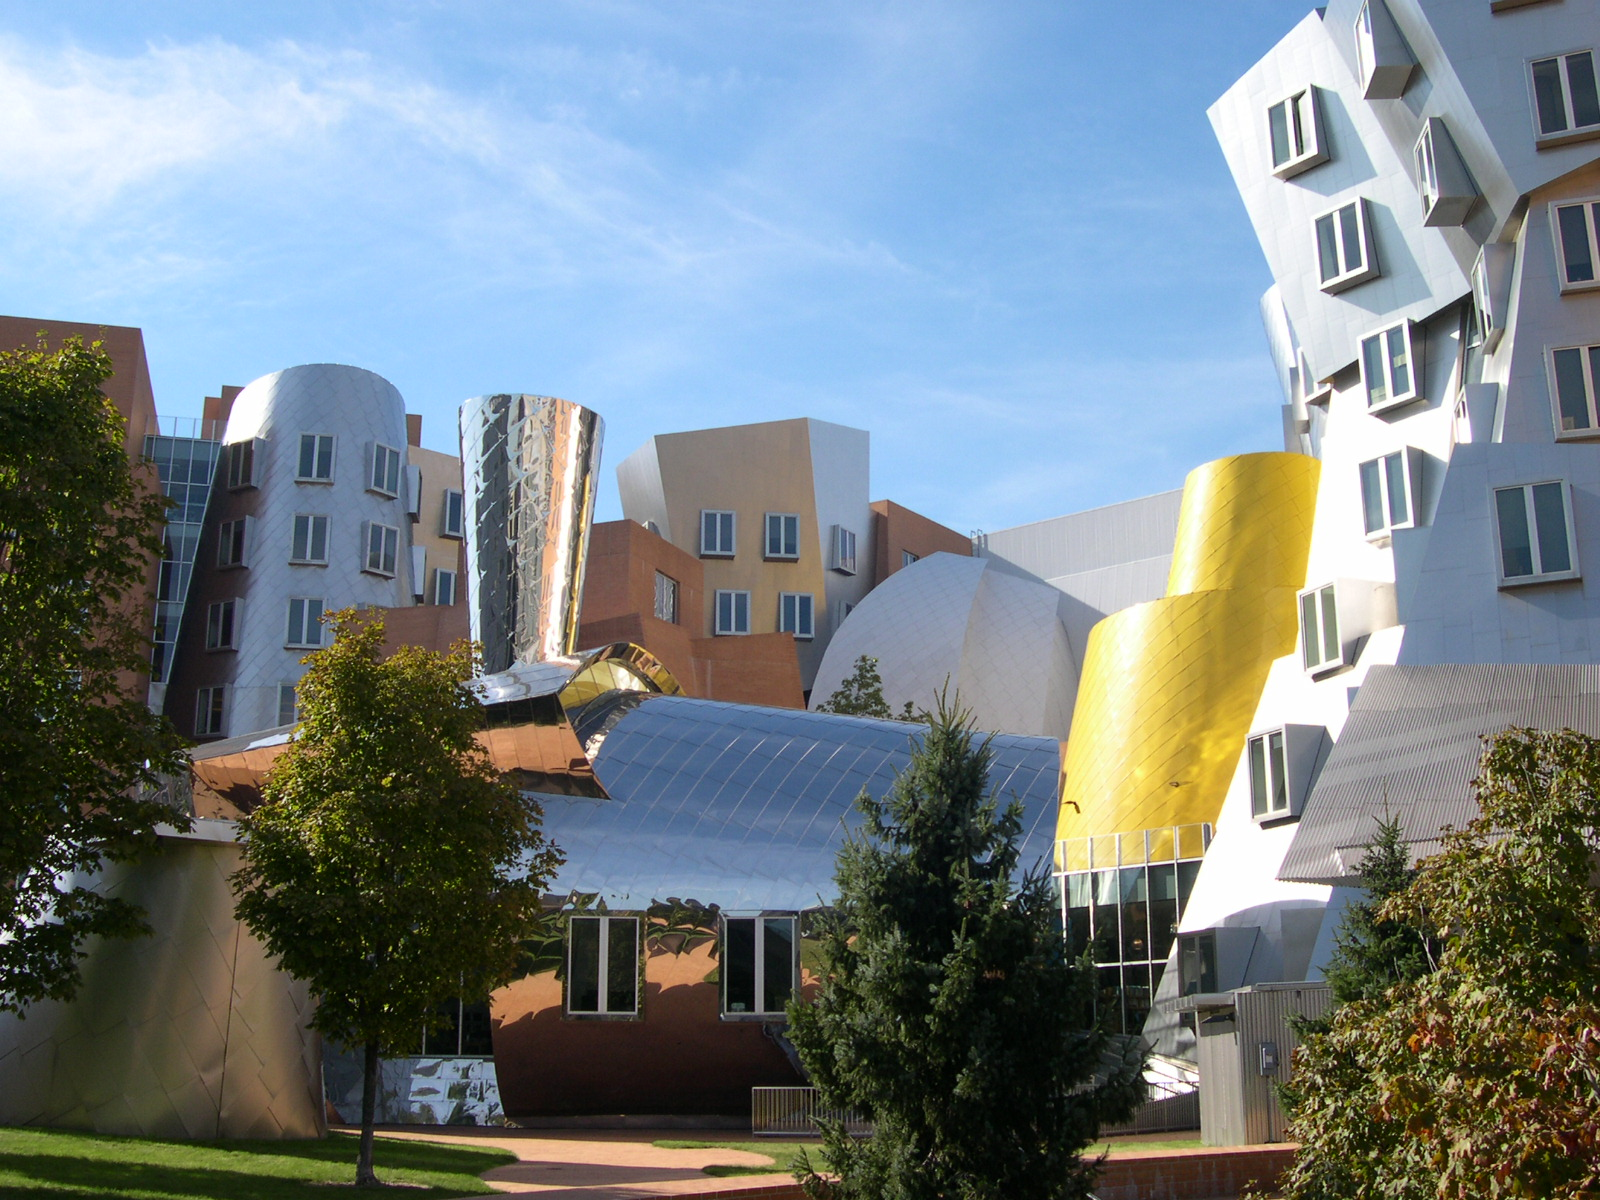
\includegraphics[width=0.8\linewidth]{Figures/stata1.jpg}
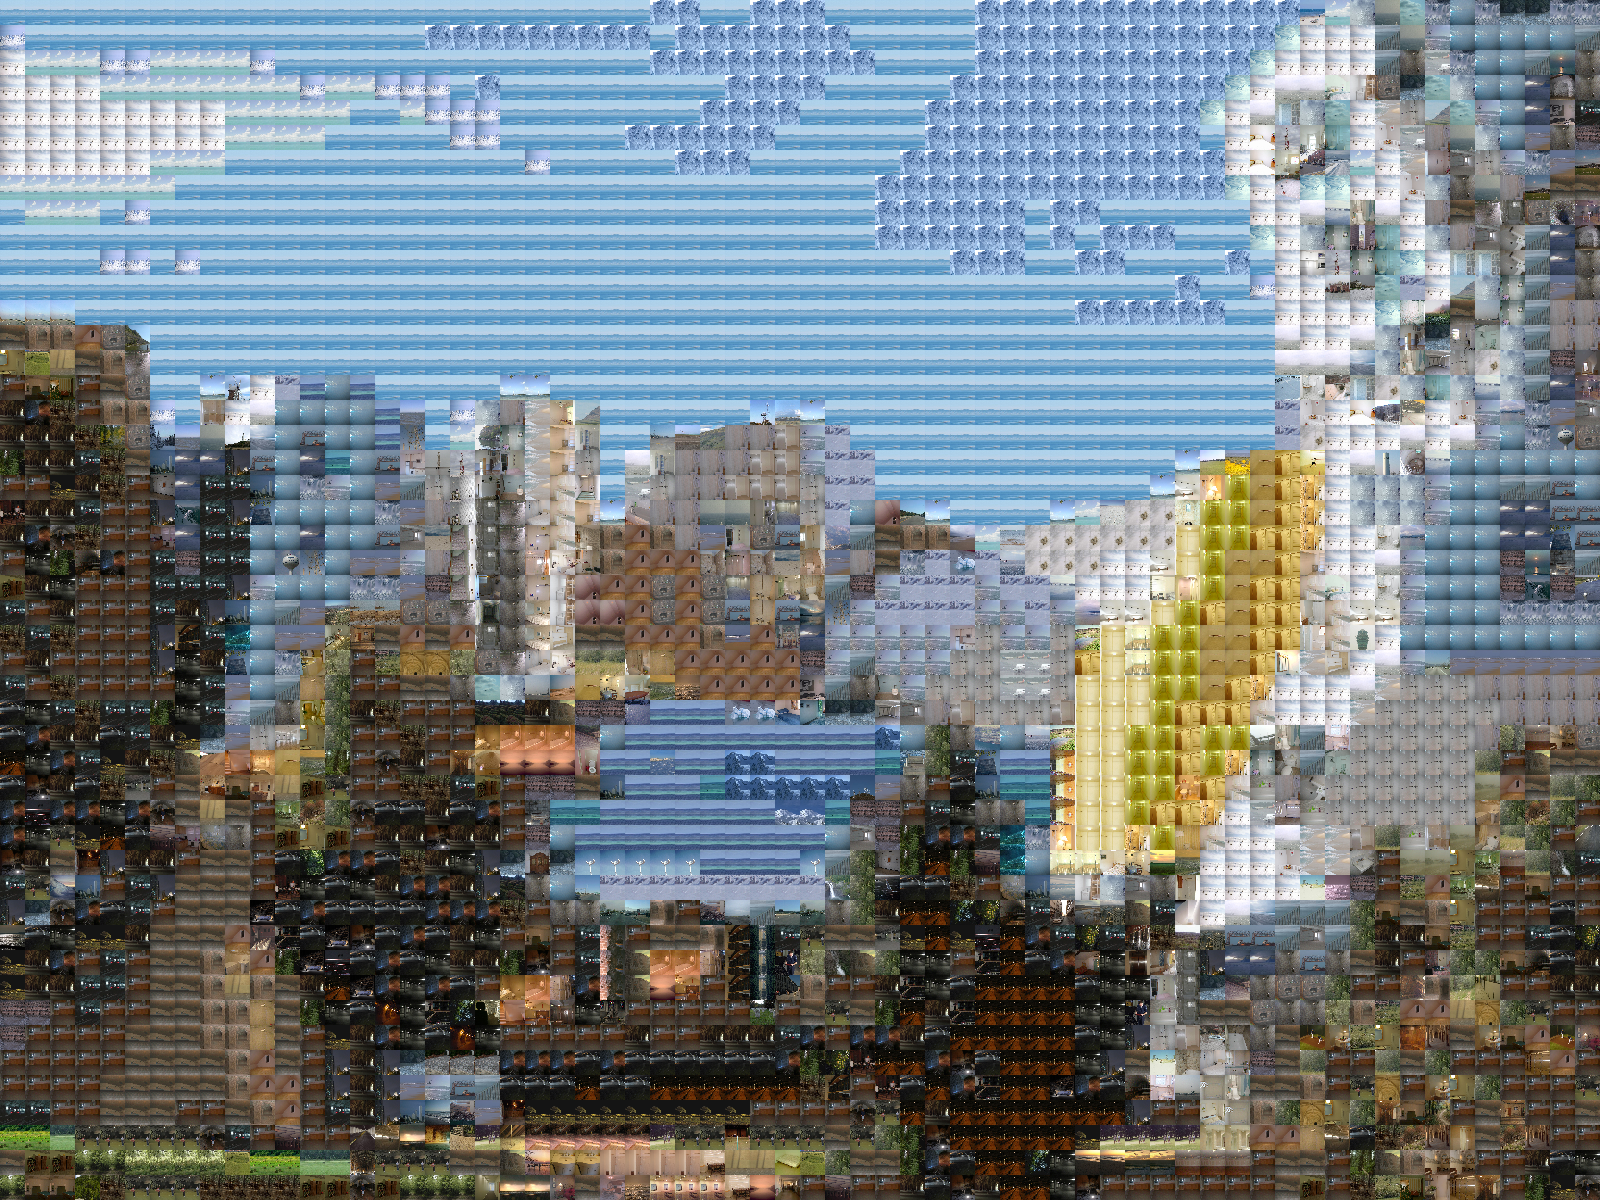
\includegraphics[width=0.8\linewidth]{Figures/saved.png}
\caption{A sample photomosaic automatically generated by our system, with only a few small modifications as described in \ref{sec:photo}.}
\label{fig:stata}
\end{figure*}

\end{document}
